\pdfoutput=1
%% Author: PGL  Porta Mana
%% Created: 2015-05-01T20:53:34+0200
%% Last-Updated: 2019-02-28T13:39:20+0100
%%%%%%%%%%%%%%%%%%%%%%%%%%%%%%%%%%%%%%%%%%%%%%%%%%%%%%%%%%%%%%%%%%%%%%%%%%%%
\newif\ifarxiv
\arxivfalse
\ifarxiv\pdfmapfile{+classico.map}\fi
\newif\ifafour
\afourfalse% true = A4, false = A5
\newif\iftypodisclaim % typographical disclaim on the side
\typodisclaimtrue
\newcommand*{\memfontfamily}{zplx}
\newcommand*{\memfontpack}{newpxtext}
\documentclass[\ifafour a4paper,12pt,\else a5paper,10pt,\fi%extrafontsizes,%
onecolumn,oneside,article,%french,italian,german,swedish,latin,
british%
]{memoir}
\newcommand*{\updated}{\today}
\newcommand*{\firstdraft}{18 April 2017}
\newcommand*{\firstpublished}{***}
\newcommand*{\propertitle}{The beauty of Grassmann spaces}
\newcommand*{\pdftitle}{\propertitle}
\newcommand*{\headtitle}{\propertitle}
\newcommand*{\pdfauthor}{I. Bengtsson, P.G.L.  Porta Mana}
\newcommand*{\headauthor}{Bengtsson \amp\ Porta Mana}
\newcommand*{\reporthead}{}
%%%%%%%%%%%%%%%%%%%%%%%%%%%%%%%%%%%%%%%%%%%%%%%%%%%%%%%%%%%%%%%%%%%%%%%%%%%%
%%% Calls to packages (uncomment as needed)
%%%%%%%%%%%%%%%%%%%%%%%%%%%%%%%%%%%%%%%%%%%%%%%%%%%%%%%%%%%%%%%%%%%%%%%%%%%%

%\usepackage{pifont}

%\usepackage{fontawesome}

\usepackage[T1]{fontenc} 
\input{glyphtounicode} \pdfgentounicode=1

\usepackage[utf8]{inputenx}

%\usepackage{newunicodechar}
% \newunicodechar{Ĕ}{\u{E}}
% \newunicodechar{ĕ}{\u{e}}
% \newunicodechar{Ĭ}{\u{I}}
% \newunicodechar{ĭ}{\u{\i}}
% \newunicodechar{Ŏ}{\u{O}}
% \newunicodechar{ŏ}{\u{o}}
% \newunicodechar{Ŭ}{\u{U}}
% \newunicodechar{ŭ}{\u{u}}
% \newunicodechar{Ā}{\=A}
% \newunicodechar{ā}{\=a}
% \newunicodechar{Ē}{\=E}
% \newunicodechar{ē}{\=e}
% \newunicodechar{Ī}{\=I}
% \newunicodechar{ī}{\={\i}}
% \newunicodechar{Ō}{\=O}
% \newunicodechar{ō}{\=o}
% \newunicodechar{Ū}{\=U}
% \newunicodechar{ū}{\=u}
% \newunicodechar{Ȳ}{\=Y}
% \newunicodechar{ȳ}{\=y}

\newcommand*{\bmmax}{0} % reduce number of bold fonts, before font packages
\newcommand*{\hmmax}{0} % reduce number of heavy fonts, before font packages

\usepackage{textcomp}

%\usepackage[normalem]{ulem}% package for underlining
% \makeatletter
% \def\ssout{\bgroup \ULdepth=-.35ex%\UL@setULdepth
%  \markoverwith{\lower\ULdepth\hbox
%    {\kern-.03em\vbox{\hrule width.2em\kern1.2\p@\hrule}\kern-.03em}}%
%  \ULon}
% \makeatother

\usepackage{amsmath}

\usepackage{mathtools}
\addtolength{\jot}{\jot} % increase spacing in multiline formulae
\setlength{\multlinegap}{0pt}

%\usepackage{empheq}% automatically calls amsmath and mathtools
\newcommand*{\widefbox}[1]{\fbox{\hspace{1em}#1\hspace{1em}}}

%\usepackage{fancybox}

%\usepackage{framed}

% \usepackage[misc]{ifsym} % for dice
% \newcommand*{\diceone}{{\scriptsize\Cube{1}}}

\usepackage{amssymb}

\usepackage{amsxtra}

\usepackage[main=british,french,italian,german,swedish,latin,esperanto]{babel}\selectlanguage{british}
\newcommand*{\langfrench}{\foreignlanguage{french}}
\newcommand*{\langgerman}{\foreignlanguage{german}}
\newcommand*{\langitalian}{\foreignlanguage{italian}}
\newcommand*{\langswedish}{\foreignlanguage{swedish}}
\newcommand*{\langlatin}{\foreignlanguage{latin}}
\newcommand*{\langnohyph}{\foreignlanguage{nohyphenation}}

\usepackage[autostyle=false,autopunct=false,english=british]{csquotes}
\setquotestyle{british}

\usepackage{amsthm}
\newcommand*{\QED}{\textsc{q.e.d.}}
\renewcommand*{\qedsymbol}{\QED}
\theoremstyle{remark}
\newtheorem{note}{Note}
\newtheorem*{remark}{Note}
\newtheoremstyle{innote}{\parsep}{\parsep}{\footnotesize}{}{}{}{0pt}{}
\theoremstyle{innote}
\newtheorem*{innote}{}

\usepackage[shortlabels,inline]{enumitem}
\SetEnumitemKey{para}{itemindent=\parindent,leftmargin=0pt,listparindent=\parindent,parsep=0pt,itemsep=\topsep}
% \begin{asparaenum} = \begin{enumerate}[para]
% \begin{inparaenum} = \begin{enumerate*}
\setlist[enumerate,2]{label=\alph*.}
\setlist[enumerate]{label=\arabic*.,leftmargin=1.5\parindent}
\setlist[itemize]{leftmargin=1.5\parindent}
\setlist[description]{leftmargin=1.5\parindent}
% old alternative:
% \setlist[enumerate,2]{label=\alph*.}
% \setlist[enumerate]{leftmargin=\parindent}
% \setlist[itemize]{leftmargin=\parindent}
% \setlist[description]{leftmargin=\parindent}

\usepackage[babel,theoremfont,largesc]{newpxtext}

\usepackage[bigdelims,nosymbolsc%,smallerops % probably arXiv doesn't have it
]{newpxmath}
\useosf\linespread{1.083}
%% smaller operators for old version of newpxmath
\makeatletter
\def\re@DeclareMathSymbol#1#2#3#4{%
    \let#1=\undefined
    \DeclareMathSymbol{#1}{#2}{#3}{#4}}
%\re@DeclareMathSymbol{\bigsqcupop}{\mathop}{largesymbols}{"46}
%\re@DeclareMathSymbol{\bigodotop}{\mathop}{largesymbols}{"4A}
\re@DeclareMathSymbol{\bigoplusop}{\mathop}{largesymbols}{"4C}
\re@DeclareMathSymbol{\bigotimesop}{\mathop}{largesymbols}{"4E}
\re@DeclareMathSymbol{\sumop}{\mathop}{largesymbols}{"50}
\re@DeclareMathSymbol{\prodop}{\mathop}{largesymbols}{"51}
\re@DeclareMathSymbol{\bigcupop}{\mathop}{largesymbols}{"53}
\re@DeclareMathSymbol{\bigcapop}{\mathop}{largesymbols}{"54}
%\re@DeclareMathSymbol{\biguplusop}{\mathop}{largesymbols}{"55}
\re@DeclareMathSymbol{\bigwedgeop}{\mathop}{largesymbols}{"56}
\re@DeclareMathSymbol{\bigveeop}{\mathop}{largesymbols}{"57}
%\re@DeclareMathSymbol{\bigcupdotop}{\mathop}{largesymbols}{"DF}
%\re@DeclareMathSymbol{\bigcapplusop}{\mathop}{largesymbolsPXA}{"00}
%\re@DeclareMathSymbol{\bigsqcupplusop}{\mathop}{largesymbolsPXA}{"02}
%\re@DeclareMathSymbol{\bigsqcapplusop}{\mathop}{largesymbolsPXA}{"04}
%\re@DeclareMathSymbol{\bigsqcapop}{\mathop}{largesymbolsPXA}{"06}
\re@DeclareMathSymbol{\bigtimesop}{\mathop}{largesymbolsPXA}{"10}
%\re@DeclareMathSymbol{\coprodop}{\mathop}{largesymbols}{"60}
%\re@DeclareMathSymbol{\varprod}{\mathop}{largesymbolsPXA}{16}
\makeatother
%%
%% With euler font cursive for Greek letters - the [1] means 100% scaling
\DeclareFontFamily{U}{egreek}{\skewchar\font'177}%
\DeclareFontShape{U}{egreek}{m}{n}{<-6>s*[1]eurm5 <6-8>s*[1]eurm7 <8->s*[1]eurm10}{}%
\DeclareFontShape{U}{egreek}{m}{it}{<->s*[1]eurmo10}{}%
\DeclareFontShape{U}{egreek}{b}{n}{<-6>s*[1]eurb5 <6-8>s*[1]eurb7 <8->s*[1]eurb10}{}%
\DeclareFontShape{U}{egreek}{b}{it}{<->s*[1]eurbo10}{}%
\DeclareSymbolFont{egreeki}{U}{egreek}{m}{it}%
\SetSymbolFont{egreeki}{bold}{U}{egreek}{b}{it}% from the amsfonts package
\DeclareSymbolFont{egreekr}{U}{egreek}{m}{n}%
\SetSymbolFont{egreekr}{bold}{U}{egreek}{b}{n}% from the amsfonts package
% Take also \sum, \prod, \coprod symbols from Euler fonts
\DeclareFontFamily{U}{egreekx}{\skewchar\font'177}
\DeclareFontShape{U}{egreekx}{m}{n}{%
       <-7.5>s*[0.9]euex7%
    <7.5-8.5>s*[0.9]euex8%
    <8.5-9.5>s*[0.9]euex9%
    <9.5->s*[0.9]euex10%
}{}
\DeclareSymbolFont{egreekx}{U}{egreekx}{m}{n}
\DeclareMathSymbol{\sumop}{\mathop}{egreekx}{"50}
\DeclareMathSymbol{\prodop}{\mathop}{egreekx}{"51}
\DeclareMathSymbol{\coprodop}{\mathop}{egreekx}{"60}
\makeatletter
\def\sum{\DOTSI\sumop\slimits@}
\def\prod{\DOTSI\prodop\slimits@}
\def\coprod{\DOTSI\coprodop\slimits@}
\makeatother
% Greek letters not usually given in LaTeX.
\DeclareMathSymbol{\varpartial}{\mathalpha}{egreeki}{"40}
\DeclareMathSymbol{\partialup}{\mathalpha}{egreekr}{"40}
\DeclareMathSymbol{\alpha}{\mathalpha}{egreeki}{"0B}
\DeclareMathSymbol{\beta}{\mathalpha}{egreeki}{"0C}
\DeclareMathSymbol{\gamma}{\mathalpha}{egreeki}{"0D}
\DeclareMathSymbol{\delta}{\mathalpha}{egreeki}{"0E}
\DeclareMathSymbol{\epsilon}{\mathalpha}{egreeki}{"0F}
\DeclareMathSymbol{\zeta}{\mathalpha}{egreeki}{"10}
\DeclareMathSymbol{\eta}{\mathalpha}{egreeki}{"11}
\DeclareMathSymbol{\theta}{\mathalpha}{egreeki}{"12}
\DeclareMathSymbol{\iota}{\mathalpha}{egreeki}{"13}
\DeclareMathSymbol{\kappa}{\mathalpha}{egreeki}{"14}
\DeclareMathSymbol{\lambda}{\mathalpha}{egreeki}{"15}
\DeclareMathSymbol{\mu}{\mathalpha}{egreeki}{"16}
\DeclareMathSymbol{\nu}{\mathalpha}{egreeki}{"17}
\DeclareMathSymbol{\xi}{\mathalpha}{egreeki}{"18}
\DeclareMathSymbol{\omicron}{\mathalpha}{egreeki}{"6F}
\DeclareMathSymbol{\pi}{\mathalpha}{egreeki}{"19}
\DeclareMathSymbol{\rho}{\mathalpha}{egreeki}{"1A}
\DeclareMathSymbol{\sigma}{\mathalpha}{egreeki}{"1B}
 \DeclareMathSymbol{\tau}{\mathalpha}{egreeki}{"1C}
\DeclareMathSymbol{\upsilon}{\mathalpha}{egreeki}{"1D}
\DeclareMathSymbol{\phi}{\mathalpha}{egreeki}{"1E}
\DeclareMathSymbol{\chi}{\mathalpha}{egreeki}{"1F}
\DeclareMathSymbol{\psi}{\mathalpha}{egreeki}{"20}
\DeclareMathSymbol{\omega}{\mathalpha}{egreeki}{"21}
\DeclareMathSymbol{\varepsilon}{\mathalpha}{egreeki}{"22}
\DeclareMathSymbol{\vartheta}{\mathalpha}{egreeki}{"23}
\DeclareMathSymbol{\varpi}{\mathalpha}{egreeki}{"24}
\let\varrho\rho 
\let\varsigma\sigma
 \let\varkappa\kappa
\DeclareMathSymbol{\varphi}{\mathalpha}{egreeki}{"27}
%
\DeclareMathSymbol{\varAlpha}{\mathalpha}{egreeki}{"41}
\DeclareMathSymbol{\varBeta}{\mathalpha}{egreeki}{"42}
\DeclareMathSymbol{\varGamma}{\mathalpha}{egreeki}{"00}
\DeclareMathSymbol{\varDelta}{\mathalpha}{egreeki}{"01}
\DeclareMathSymbol{\varEpsilon}{\mathalpha}{egreeki}{"45}
\DeclareMathSymbol{\varZeta}{\mathalpha}{egreeki}{"5A}
\DeclareMathSymbol{\varEta}{\mathalpha}{egreeki}{"48}
\DeclareMathSymbol{\varTheta}{\mathalpha}{egreeki}{"02}
 \DeclareMathSymbol{\varIota}{\mathalpha}{egreeki}{"49}
\DeclareMathSymbol{\varKappa}{\mathalpha}{egreeki}{"4B}
\DeclareMathSymbol{\varLambda}{\mathalpha}{egreeki}{"03}
\DeclareMathSymbol{\varMu}{\mathalpha}{egreeki}{"4D}
\DeclareMathSymbol{\varNu}{\mathalpha}{egreeki}{"4E}
\DeclareMathSymbol{\varXi}{\mathalpha}{egreeki}{"04}
\DeclareMathSymbol{\varOmicron}{\mathalpha}{egreeki}{"4F}
\DeclareMathSymbol{\varPi}{\mathalpha}{egreeki}{"05}
\DeclareMathSymbol{\varRho}{\mathalpha}{egreeki}{"50}
\DeclareMathSymbol{\varSigma}{\mathalpha}{egreeki}{"06}
\DeclareMathSymbol{\varTau}{\mathalpha}{egreeki}{"54}
\DeclareMathSymbol{\varUpsilon}{\mathalpha}{egreeki}{"07}
\DeclareMathSymbol{\varPhi}{\mathalpha}{egreeki}{"08}
\DeclareMathSymbol{\varChi}{\mathalpha}{egreeki}{"58}
\DeclareMathSymbol{\varPsi}{\mathalpha}{egreeki}{"09}
\DeclareMathSymbol{\varOmega}{\mathalpha}{egreeki}{"0A} 
%
\DeclareMathSymbol{\Alpha}{\mathalpha}{egreekr}{"41}
\DeclareMathSymbol{\Beta}{\mathalpha}{egreekr}{"42}
\DeclareMathSymbol{\Gamma}{\mathalpha}{egreekr}{"00}
\DeclareMathSymbol{\Delta}{\mathalpha}{egreekr}{"01}
\DeclareMathSymbol{\Epsilon}{\mathalpha}{egreekr}{"45}
\DeclareMathSymbol{\Zeta}{\mathalpha}{egreekr}{"5A}
\DeclareMathSymbol{\Eta}{\mathalpha}{egreekr}{"48}
\DeclareMathSymbol{\Theta}{\mathalpha}{egreekr}{"02}
\DeclareMathSymbol{\Iota}{\mathalpha}{egreekr}{"49}
\DeclareMathSymbol{\Kappa}{\mathalpha}{egreekr}{"4B}
\DeclareMathSymbol{\Lambda}{\mathalpha}{egreekr}{"03}
\DeclareMathSymbol{\Mu}{\mathalpha}{egreekr}{"4D}
\DeclareMathSymbol{\Nu}{\mathalpha}{egreekr}{"4E}
\DeclareMathSymbol{\Xi}{\mathalpha}{egreekr}{"04}
\DeclareMathSymbol{\Omicron}{\mathalpha}{egreekr}{"4F}
\DeclareMathSymbol{\Pi}{\mathalpha}{egreekr}{"05}
\DeclareMathSymbol{\Rho}{\mathalpha}{egreekr}{"50}
\DeclareMathSymbol{\Sigma}{\mathalpha}{egreekr}{"06}
\DeclareMathSymbol{\Tau}{\mathalpha}{egreekr}{"54}
\DeclareMathSymbol{\Upsilon}{\mathalpha}{egreekr}{"07}
\DeclareMathSymbol{\Phi}{\mathalpha}{egreekr}{"08}
\DeclareMathSymbol{\Chi}{\mathalpha}{egreekr}{"58}
\DeclareMathSymbol{\Psi}{\mathalpha}{egreekr}{"09}
\DeclareMathSymbol{\Omega}{\mathalpha}{egreekr}{"0A}
%
\DeclareMathSymbol{\alphaup}{\mathalpha}{egreekr}{"0B}
\DeclareMathSymbol{\betaup}{\mathalpha}{egreekr}{"0C}
\DeclareMathSymbol{\gammaup}{\mathalpha}{egreekr}{"0D}
 \DeclareMathSymbol{\deltaup}{\mathalpha}{egreekr}{"0E}
\DeclareMathSymbol{\epsilonup}{\mathalpha}{egreekr}{"0F}
\DeclareMathSymbol{\zetaup}{\mathalpha}{egreekr}{"10}
\DeclareMathSymbol{\etaup}{\mathalpha}{egreekr}{"11}
\DeclareMathSymbol{\thetaup}{\mathalpha}{egreekr}{"12}
\DeclareMathSymbol{\iotaup}{\mathalpha}{egreekr}{"13}
\DeclareMathSymbol{\kappaup}{\mathalpha}{egreekr}{"14}
\DeclareMathSymbol{\lambdaup}{\mathalpha}{egreekr}{"15}
\DeclareMathSymbol{\muup}{\mathalpha}{egreekr}{"16}
\DeclareMathSymbol{\nuup}{\mathalpha}{egreekr}{"17}
\DeclareMathSymbol{\xiup}{\mathalpha}{egreekr}{"18}
\DeclareMathSymbol{\omicronup}{\mathalpha}{egreekr}{"6F}
  \DeclareMathSymbol{\piup}{\mathalpha}{egreekr}{"19}
\DeclareMathSymbol{\rhoup}{\mathalpha}{egreekr}{"1A}
\DeclareMathSymbol{\sigmaup}{\mathalpha}{egreekr}{"1B}
\DeclareMathSymbol{\tauup}{\mathalpha}{egreekr}{"1C}
\DeclareMathSymbol{\upsilonup}{\mathalpha}{egreekr}{"1D}
\DeclareMathSymbol{\phiup}{\mathalpha}{egreekr}{"1E}
\DeclareMathSymbol{\chiup}{\mathalpha}{egreekr}{"1F}
\DeclareMathSymbol{\psiup}{\mathalpha}{egreekr}{"20}
\DeclareMathSymbol{\omegaup}{\mathalpha}{egreekr}{"21}
\DeclareMathSymbol{\varepsilonup}{\mathalpha}{egreekr}{"22}
\DeclareMathSymbol{\varthetaup}{\mathalpha}{egreekr}{"23}
\DeclareMathSymbol{\varpiup}{\mathalpha}{egreekr}{"24}
\let\varrhoup\rhoup 
\let\varsigmaup\sigmaup
\let\varkappaup\kappaup
\DeclareMathSymbol{\varphiup}{\mathalpha}{egreekr}{"27}
% Greek letters not usually given in LaTeX.

%\usepackage%[scaled=0.9]%
%{classico}%  Optima as sans-serif font
\renewcommand\sfdefault{uop}
\DeclareMathAlphabet{\mathsf}  {T1}{\sfdefault}{m}{sl}
\SetMathAlphabet{\mathsf}{bold}{T1}{\sfdefault}{b}{sl}
%\newcommand*{\mathte}[1]{\textbf{\textit{\textsf{#1}}}}
% Upright sans-serif math alphabet
% \DeclareMathAlphabet{\mathsu}  {T1}{\sfdefault}{m}{n}
% \SetMathAlphabet{\mathsu}{bold}{T1}{\sfdefault}{b}{n}

% DejaVu Mono as typewriter text
\usepackage[scaled=0.84]{DejaVuSansMono}

\usepackage{mathdots}

\usepackage[usenames]{xcolor}
% Tol (2012) colour-blind-, print-, screen-friendly colours, alternative scheme; Munsell terminology
\definecolor{mypurpleblue}{RGB}{68,119,170}
\definecolor{myblue}{RGB}{102,204,238}
\definecolor{mygreen}{RGB}{34,136,51}
\definecolor{myyellow}{RGB}{204,187,68}
\definecolor{myred}{RGB}{238,102,119}
\definecolor{myredpurple}{RGB}{170,51,119}
\definecolor{mygrey}{RGB}{187,187,187}
% Tol (2012) colour-blind-, print-, screen-friendly colours; Munsell terminology
% \definecolor{lbpurple}{RGB}{51,34,136}
% \definecolor{lblue}{RGB}{136,204,238}
% \definecolor{lbgreen}{RGB}{68,170,153}
% \definecolor{lgreen}{RGB}{17,119,51}
% \definecolor{lgyellow}{RGB}{153,153,51}
% \definecolor{lyellow}{RGB}{221,204,119}
% \definecolor{lred}{RGB}{204,102,119}
% \definecolor{lpred}{RGB}{136,34,85}
% \definecolor{lrpurple}{RGB}{170,68,153}
\definecolor{lgrey}{RGB}{221,221,221}
%\newcommand*\mycolourbox[1]{%
%\colorbox{mygrey}{\hspace{1em}#1\hspace{1em}}}
\colorlet{shadecolor}{lgrey}

\usepackage{bm}

\usepackage{microtype}

\usepackage[backend=biber,mcite,%subentry,
citestyle=authoryear-comp,bibstyle=pglpm-authoryear,autopunct=false,sorting=ny,sortcites=false,natbib=false,maxcitenames=1,maxbibnames=8,minbibnames=8,giveninits=true,uniquename=false,uniquelist=false,maxalphanames=1,block=space,hyperref=true,defernumbers=false,useprefix=true,sortupper=false,language=british,parentracker=false]{biblatex}
\DeclareSortingScheme{ny}{\sort{\field{sortname}\field{author}\field{editor}}\sort{\field{year}}}
\iffalse\makeatletter%%% replace parenthesis with brackets
\newrobustcmd*{\parentexttrack}[1]{%
  \begingroup
  \blx@blxinit
  \blx@setsfcodes
  \blx@bibopenparen#1\blx@bibcloseparen
  \endgroup}
\AtEveryCite{%
  \let\parentext=\parentexttrack%
  \let\bibopenparen=\bibopenbracket%
  \let\bibcloseparen=\bibclosebracket}
\makeatother\fi
\DefineBibliographyExtras{british}{\def\finalandcomma{\addcomma}}
\renewcommand*{\finalnamedelim}{\addcomma\space}
\setcounter{biburlnumpenalty}{1}
\setcounter{biburlucpenalty}{0}
\setcounter{biburllcpenalty}{1}
\DeclareDelimFormat{multicitedelim}{\addsemicolon\space}
\DeclareDelimFormat{compcitedelim}{\addsemicolon\space}
\DeclareDelimFormat{postnotedelim}{\space}
\ifarxiv\else\addbibresource{portamanabib.bib}\fi
\renewcommand{\bibfont}{\footnotesize}
%\appto{\citesetup}{\footnotesize}% smaller font for citations
\defbibheading{bibliography}[\bibname]{\section*{#1}\addcontentsline{toc}{section}{#1}%\markboth{#1}{#1}
}
\newcommand*{\citep}{\parencites}
\newcommand*{\citey}{\parencites*}
%\renewcommand*{\cite}{\parencite}
\renewcommand*{\cites}{\parencites}
\providecommand{\href}[2]{#2}
\providecommand{\eprint}[2]{\texttt{\href{#1}{#2}}}
\newcommand*{\amp}{\&}
% \newcommand*{\citein}[2][]{\textnormal{\textcite[#1]{#2}}%\addtocategory{extras}{#2}
% }
\newcommand*{\citein}[2][]{\textnormal{\textcite[#1]{#2}}%\addtocategory{extras}{#2}
}
\newcommand*{\citebi}[2][]{\textcite[#1]{#2}%\addtocategory{extras}{#2}
}
\newcommand*{\subtitleproc}[1]{}
\newcommand*{\chapb}{ch.}
%
% \def\arxivp{}
% \def\mparcp{}
% \def\philscip{}
% \def\biorxivp{}
% \newcommand*{\arxivsi}{\texttt{arXiv} eprints available at \url{http://arxiv.org/}.\\}
% \newcommand*{\mparcsi}{\texttt{mp\_arc} eprints available at \url{http://www.ma.utexas.edu/mp_arc/}.\\}
% \newcommand*{\philscisi}{\texttt{philsci} eprints available at \url{http://philsci-archive.pitt.edu/}.\\}
% \newcommand*{\biorxivsi}{\texttt{bioRxiv} eprints available at \url{http://biorxiv.org/}.\\}
\newcommand*{\arxiveprint}[1]{%\global\def\arxivp{\arxivsi}%\citeauthor{0arxivcite}\addtocategory{ifarchcit}{0arxivcite}%eprint
\texttt{\urlalt{https://arxiv.org/abs/#1}{arXiv:\hspace{0pt}#1}}%
%\texttt{\href{http://arxiv.org/abs/#1}{\protect\url{arXiv:#1}}}%
%\renewcommand{\arxivnote}{\texttt{arXiv} eprints available at \url{http://arxiv.org/}.}
}
\newcommand*{\mparceprint}[1]{%\global\def\mparcp{\mparcsi}%\citeauthor{0mparccite}\addtocategory{ifarchcit}{0mparccite}%eprint
\texttt{\urlalt{http://www.ma.utexas.edu/mp_arc-bin/mpa?yn=#1}{mp\_arc:\hspace{0pt}#1}}%
%\texttt{\href{http://www.ma.utexas.edu/mp_arc-bin/mpa?yn=#1}{\protect\url{mp_arc:#1}}}%
%\providecommand{\mparcnote}{\texttt{mp_arc} eprints available at \url{http://www.ma.utexas.edu/mp_arc/}.}
}
\newcommand*{\philscieprint}[1]{%\global\def\philscip{\philscisi}%\citeauthor{0philscicite}\addtocategory{ifarchcit}{0philscicite}%eprint
\texttt{\urlalt{http://philsci-archive.pitt.edu/archive/#1}{PhilSci:\hspace{0pt}#1}}%
%\texttt{\href{http://philsci-archive.pitt.edu/archive/#1}{\protect\url{PhilSci:#1}}}%
%\providecommand{\mparcnote}{\texttt{philsci} eprints available at \url{http://philsci-archive.pitt.edu/}.}
}
\newcommand*{\biorxiveprint}[1]{%\global\def\biorxivp{\biorxivsi}%\citeauthor{0arxivcite}\addtocategory{ifarchcit}{0arxivcite}%eprint
\texttt{\urlalt{https://doi.org/10.1101/#1}{bioRxiv doi:\hspace{0pt}10.1101/#1}}%
%\texttt{\href{http://arxiv.org/abs/#1}{\protect\url{arXiv:#1}}}%
%\renewcommand{\arxivnote}{\texttt{arXiv} eprints available at \url{http://arxiv.org/}.}
}
\newcommand*{\osfeprint}[1]{%
\texttt{\urlalt{https://doi.org/10.17605/osf.io/#1}{Open Science Framework doi:10.17605/osf.io/#1}}%
}

\usepackage{graphicx}

%\usepackage{wrapfig}

%\usepackage{tikz-cd}

\PassOptionsToPackage{hyphens}{url}\usepackage[hypertexnames=false]{hyperref}

\usepackage[depth=4]{bookmark}
\hypersetup{colorlinks=true,bookmarksnumbered,pdfborder={0 0 0.25},citebordercolor={0.2667 0.4667 0.6667},citecolor=mypurpleblue,linkbordercolor={0.6667 0.2 0.4667},linkcolor=myredpurple,urlbordercolor={0.1333 0.5333 0.2},urlcolor=mygreen,breaklinks=true,pdftitle={\pdftitle},pdfauthor={\pdfauthor}}
% \usepackage[vertfit=local]{breakurl}% only for arXiv
\providecommand*{\urlalt}{\href}

\usepackage[british]{datetime2}
\DTMnewdatestyle{mydate}%
{% definitions
\renewcommand*{\DTMdisplaydate}[4]{%
\number##3\ \DTMenglishmonthname{##2} ##1}%
\renewcommand*{\DTMDisplaydate}{\DTMdisplaydate}%
}
\DTMsetdatestyle{mydate}

%%%%%%%%%%%%%%%%%%%%%%%%%%%%%%%%%%%%%%%%%%%%%%%%%%%%%%%%%%%%%%%%%%%%%%%%%%%%
%%% Layout. I do not know on which kind of paper the reader will print the
%%% paper on (A4? letter? one-sided? double-sided?). So I choose A5, which
%%% provides a good layout for reading on screen and save paper if printed
%%% two pages per sheet. Average length line is 66 characters and page
%%% numbers are centred.
%%%%%%%%%%%%%%%%%%%%%%%%%%%%%%%%%%%%%%%%%%%%%%%%%%%%%%%%%%%%%%%%%%%%%%%%%%%%
\ifafour\setstocksize{297mm}{210mm}%{*}% A4
\else\setstocksize{210mm}{5.5in}%{*}% 210x139.7
\fi
\settrimmedsize{\stockheight}{\stockwidth}{*}
\setlxvchars[\normalfont] %313.3632pt for a 66-characters line
\setxlvchars[\normalfont]
\setlength{\trimtop}{0pt}
\setlength{\trimedge}{\stockwidth}
\addtolength{\trimedge}{-\paperwidth}
% The length of the normalsize alphabet is 133.05988pt - 10 pt = 26.1408pc
% The length of the normalsize alphabet is 159.6719pt - 12pt = 30.3586pc
% Bringhurst gives 32pc as boundary optimal with 69 ch per line
% The length of the normalsize alphabet is 191.60612pt - 14pt = 35.8634pc
\ifafour\settypeblocksize{*}{32pc}{1.618} % A4
%\setulmargins{*}{*}{1.667}%gives 5/3 margins % 2 or 1.667
\else\settypeblocksize{*}{26pc}{1.618}% nearer to a 66-line newpx and preserves GR
\fi
\setulmargins{*}{*}{1}%gives equal margins
\setlrmargins{*}{*}{*}
\setheadfoot{\onelineskip}{2.5\onelineskip}
\setheaderspaces{*}{2\onelineskip}{*}
\setmarginnotes{2ex}{10mm}{0pt}
\checkandfixthelayout[nearest]
\fixpdflayout
%%% End layout
%% this fixes missing white spaces
\pdfmapline{+dummy-space <dummy-space.pfb}\pdfinterwordspaceon%

%%% Sectioning
\newcommand*{\asudedication}[1]{%
{\par\centering\textit{#1}\par}}
\newenvironment{acknowledgements}{\section*{Thanks}\addcontentsline{toc}{section}{Thanks}}{\par}
\makeatletter\renewcommand{\appendix}{\par
  \bigskip{\centering
   \interlinepenalty \@M
   \normalfont
   \printchaptertitle{\sffamily\appendixpagename}\par}
  \setcounter{section}{0}%
  \gdef\@chapapp{\appendixname}%
  \gdef\thesection{\@Alph\c@section}%
  \anappendixtrue}\makeatother
\counterwithout{section}{chapter}
\setsecnumformat{\upshape\csname the#1\endcsname\quad}
\setsecheadstyle{\large\bfseries\sffamily%
\centering}
\setsubsecheadstyle{\bfseries\sffamily%
\raggedright}
%\setbeforesecskip{-1.5ex plus 1ex minus .2ex}% plus 1ex minus .2ex}
%\setaftersecskip{1.3ex plus .2ex }% plus 1ex minus .2ex}
%\setsubsubsecheadstyle{\bfseries\sffamily\slshape\raggedright}
%\setbeforesubsecskip{1.25ex plus 1ex minus .2ex }% plus 1ex minus .2ex}
%\setaftersubsecskip{-1em}%{-0.5ex plus .2ex}% plus 1ex minus .2ex}
\setsubsecindent{0pt}%0ex plus 1ex minus .2ex}
\setparaheadstyle{\bfseries\sffamily%
\raggedright}
\setcounter{secnumdepth}{2}
\setlength{\headwidth}{\textwidth}
\newcommand{\addchap}[1]{\chapter*[#1]{#1}\addcontentsline{toc}{chapter}{#1}}
\newcommand{\addsec}[1]{\section*{#1}\addcontentsline{toc}{section}{#1}}
\newcommand{\addsubsec}[1]{\subsection*{#1}\addcontentsline{toc}{subsection}{#1}}
\newcommand{\addpara}[1]{\paragraph*{#1.}\addcontentsline{toc}{subsubsection}{#1}}
\newcommand{\addparap}[1]{\paragraph*{#1}\addcontentsline{toc}{subsubsection}{#1}}

%%% Headers, footers, pagestyle
\copypagestyle{manaart}{plain}
\makeheadrule{manaart}{\headwidth}{0.5\normalrulethickness}
\makeoddhead{manaart}{%
{\footnotesize%\sffamily%
\scshape\headauthor}}{}{{\footnotesize\sffamily%
\headtitle}}
\makeoddfoot{manaart}{}{\thepage}{}
\newcommand*\autanet{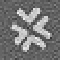
\includegraphics[height=\heightof{M}]{autanet.pdf}}
\definecolor{mygray}{gray}{0.333}
\iftypodisclaim%
\ifafour\newcommand\addprintnote{\begin{picture}(0,0)%
\put(245,149){\makebox(0,0){\rotatebox{90}{\tiny\color{mygray}\textsf{This
            document is designed for screen reading and
            two-up printing on A4 or Letter paper}}}}%
\end{picture}}% A4
\else\newcommand\addprintnote{\begin{picture}(0,0)%
\put(176,112){\makebox(0,0){\rotatebox{90}{\tiny\color{mygray}\textsf{This
            document is designed for screen reading and
            two-up printing on A4 or Letter paper}}}}%
\end{picture}}\fi%afourtrue
\makeoddfoot{plain}{}{\makebox[0pt]{\thepage}\addprintnote}{}
\else
\makeoddfoot{plain}{}{\makebox[0pt]{\thepage}}{}
\fi%typodisclaimtrue
\makeoddhead{plain}{}{}{\footnotesize\reporthead}
% \copypagestyle{manainitial}{plain}
% \makeheadrule{manainitial}{\headwidth}{0.5\normalrulethickness}
% \makeoddhead{manainitial}{%
% \footnotesize\sffamily%
% \scshape\headauthor}{}{\footnotesize\sffamily%
% \headtitle}
% \makeoddfoot{manaart}{}{\thepage}{}

\pagestyle{manaart}

\setlength{\droptitle}{-3.9\onelineskip}
\pretitle{\begin{center}\Large\sffamily%
\bfseries}
\posttitle{\bigskip\end{center}}

\makeatletter\newcommand*{\atf}{
\includegraphics[%trim=1pt 1pt 0pt 0pt,
totalheight=\heightof{@}]{atblack.png}}\makeatother
\providecommand{\affiliation}[1]{\textsl{\textsf{\footnotesize #1}}}
\providecommand{\epost}[1]{\texttt{\footnotesize\textless#1\textgreater}}
\providecommand{\email}[2]{\href{mailto:#1ZZ@#2 ((remove ZZ))}{#1\protect\atf#2}}

\preauthor{\vspace{-0.5\baselineskip}\begin{center}
\normalsize\sffamily%
\lineskip  0.5em}
\postauthor{\par\end{center}}
\predate{\DTMsetdatestyle{mydate}\begin{center}\footnotesize}
\postdate{\end{center}\vspace{-\medskipamount}}

\setfloatadjustment{figure}{\footnotesize}
\captiondelim{\quad}
\captionnamefont{\footnotesize\sffamily%
}
\captiontitlefont{\footnotesize}
\firmlists*
\midsloppy
% handling orphan/widow lines, memman.pdf
% \clubpenalty=10000
% \widowpenalty=10000
% \raggedbottom
% Downes, memman.pdf
\clubpenalty=9996
\widowpenalty=9999
\brokenpenalty=4991
\predisplaypenalty=10000
\postdisplaypenalty=1549
\displaywidowpenalty=1602
\selectlanguage{british}\frenchspacing

%%%%%%%%%%%%%%%%%%%%%%%%%%%%%%%%%%%%%%%%%%%%%%%%%%%%%%%%%%%%%%%%%%%%%%%%%%%%
%%% Paper's details
%%%%%%%%%%%%%%%%%%%%%%%%%%%%%%%%%%%%%%%%%%%%%%%%%%%%%%%%%%%%%%%%%%%%%%%%%%%%
\title{\propertitle%\\
%  {\large ***subtitle}%
}
\author{%
\hspace*{\stretch{1}}%
%% uncomment if additional authors present
\parbox{0.5\linewidth}%\makebox[0pt][c]%
{\protect\centering I. Bengtsson\\%
\footnotesize\epost{\email{ingemar}{fysik.su.se}}}%
\hspace*{\stretch{1}}%
\parbox{0.5\linewidth}%\makebox[0pt][c]%
{\protect\centering P.G.L.  Porta Mana\\%
\footnotesize\epost{\email{piero.mana}{ntnu.no}}}%
\hspace*{\stretch{1}}%
%\quad\href{https://orcid.org/0000-0002-6070-0784}{\protect\includegraphics[scale=0.16]{orcid_32x32.png}\textsc{orcid}:0000-0002-6070-0784}%
\\[2\jot] {\footnotesize\textnormal{\emph{line art by I. Bengtsson}}}%
}

\date{Draft of \today\ (first drafted \firstdraft)}
%\date{\firstpublished; updated \updated}

%%%%%%%%%%%%%%%%%%%%%%%%%%%%%%%%%%%%%%%%%%%%%%%%%%%%%%%%%%%%%%%%%%%%%%%%%%%%
%%% Macros @@@
%%%%%%%%%%%%%%%%%%%%%%%%%%%%%%%%%%%%%%%%%%%%%%%%%%%%%%%%%%%%%%%%%%%%%%%%%%%%

% Common ones - uncomment as needed
%\providecommand{\nequiv}{\not\equiv}
%\providecommand{\coloneqq}{\mathrel{\mathop:}=}
%\providecommand{\eqqcolon}{=\mathrel{\mathop:}}
%\providecommand{\varprod}{\prod}
\newcommand*{\de}{\partialup}%partial diff
\newcommand*{\pu}{\piup}%constant pi
\newcommand*{\delt}{\deltaup}%Kronecker, Dirac
%\newcommand*{\eps}{\varepsilonup}%Levi-Civita, Heaviside
%\newcommand*{\riem}{\zetaup}%Riemann zeta
%\providecommand{\degree}{\textdegree}% degree
%\newcommand*{\celsius}{\textcelsius}% degree Celsius
%\newcommand*{\micro}{\textmu}% degree Celsius
\newcommand*{\I}{\mathrm{i}}%imaginary unit
\newcommand*{\e}{\mathrm{e}}%Neper
\newcommand*{\di}{\mathrm{d}}%differential
%\newcommand*{\Di}{\mathrm{D}}%capital differential
%\newcommand*{\planckc}{\hslash}
%\newcommand*{\avogn}{N_{\textrm{A}}}
%\newcommand*{\NN}{\bm{\mathrm{N}}}
%\newcommand*{\ZZ}{\bm{\mathrm{Z}}}
%\newcommand*{\QQ}{\bm{\mathrm{Q}}}
\newcommand*{\RR}{\bm{\mathrm{R}}}
%\newcommand*{\CC}{\bm{\mathrm{C}}}
%\newcommand*{\nabl}{\bm{\nabla}}%nabla
%\DeclareMathOperator{\lb}{lb}%base 2 log
%\DeclareMathOperator{\tr}{tr}%trace
%\DeclareMathOperator{\card}{card}%cardinality
%\DeclareMathOperator{\im}{Im}%im part
%\DeclareMathOperator{\re}{Re}%re part
%\DeclareMathOperator{\sgn}{sgn}%signum
%\DeclareMathOperator{\ent}{ent}%integer less or equal to
%\DeclareMathOperator{\Ord}{O}%same order as
%\DeclareMathOperator{\ord}{o}%lower order than
%\newcommand*{\incr}{\triangle}%finite increment
\newcommand*{\defd}{\coloneqq}
\newcommand*{\defs}{\eqqcolon}
%\newcommand*{\Land}{\bigwedge}
%\newcommand*{\Lor}{\bigvee}
%\newcommand*{\lland}{\DOTSB\;\land\;}
%\newcommand*{\llor}{\DOTSB\;\lor\;}
%\newcommand*{\limplies}{\mathbin{\Rightarrow}}%implies
%\newcommand*{\suchthat}{\mid}%{\mathpunct{|}}%such that (eg in sets)
%\newcommand*{\with}{\colon}%with (list of indices)
%\newcommand*{\mul}{\times}%multiplication
%\newcommand*{\inn}{\cdot}%inner product
\newcommand*{\dotv}{\mathord{\,\cdot\,}}%variable place
%\newcommand*{\comp}{\circ}%composition of functions
%\newcommand*{\con}{\mathbin{:}}%scal prod of tensors
%\newcommand*{\equi}{\sim}%equivalent to 
\renewcommand*{\asymp}{\simeq}%equivalent to 
%\newcommand*{\corr}{\mathrel{\hat{=}}}%corresponds to
%\providecommand{\varparallel}{\ensuremath{\mathbin{/\mkern-7mu/}}}%parallel (tentative symbol)
\renewcommand*{\le}{\leqslant}%less or equal
\renewcommand*{\ge}{\geqslant}%greater or equal
%\DeclarePairedDelimiter\clcl{[}{]}
%\DeclarePairedDelimiter\clop{[}{[}
%\DeclarePairedDelimiter\opcl{]}{]}
%\DeclarePairedDelimiter\opop{]}{[}
\DeclarePairedDelimiter\abs{\lvert}{\rvert}
%\DeclarePairedDelimiter\norm{\lVert}{\rVert}
\DeclarePairedDelimiter\set{\{}{\}}
%\DeclareMathOperator{\pr}{P}%probability
\newcommand*{\pf}{\mathrm{p}}%probability
\newcommand*{\p}{\mathrm{P}}%probability
%\newcommand*{\E}{\mathrm{E}}
\renewcommand*{\|}{\nonscript\,\vert\nonscript\;\mathopen{}}
%\DeclarePairedDelimiterX{\cond}[2]{(}{)}{#1\nonscript\,\delimsize\vert\nonscript\;\mathopen{}#2}
%\DeclarePairedDelimiterX{\condt}[2]{[}{]}{#1\nonscript\,\delimsize\vert\nonscript\;\mathopen{}#2}
%\DeclarePairedDelimiterX{\conds}[2]{\{}{\}}{#1\nonscript\,\delimsize\vert\nonscript\;\mathopen{}#2}
%\newcommand*{\+}{\lor}
%\renewcommand{\*}{\land}
\newcommand*{\sect}{\S}% Sect.~
\newcommand*{\sects}{\S\S}% Sect.~
\newcommand*{\chap}{ch.}%
\newcommand*{\chaps}{chs}%
\newcommand*{\bref}{ref.}%
\newcommand*{\brefs}{refs}%
%\newcommand*{\fn}{fn}%
\newcommand*{\eqn}{eq.}%
\newcommand*{\eqns}{eqs}%
\newcommand*{\fig}{fig.}%
\newcommand*{\figs}{figs}%
\newcommand*{\vs}{{vs}}
\newcommand*{\etc}{{etc.}}
\newcommand*{\ie}{{i.e.}}
%\newcommand*{\ca}{{c.}}
%\newcommand*{\eg}{{e.g.}}
\newcommand*{\foll}{{ff.}}
%\newcommand*{\viz}{{viz}}
\newcommand*{\cf}{{cf.}}
%\newcommand*{\Cf}{{Cf.}}
%\newcommand*{\vd}{{v.}}
\newcommand*{\etal}{{\amp\ al.}}
%\newcommand*{\etsim}{{et sim.}}
%\newcommand*{\ibid}{{ibid.}}
%\newcommand*{\sic}{{sic}}
%\newcommand*{\id}{\mathte{I}}%id matrix
%\newcommand*{\nbd}{\nobreakdash}%
%\newcommand*{\bd}{\hspace{0pt}}%
%\def\hy{-\penalty0\hskip0pt\relax}
%\newcommand*{\labelbis}[1]{\tag*{(\ref{#1})$_\text{r}$}}
%\newcommand*{\mathbox}[2][.8]{\parbox[t]{#1\columnwidth}{#2}}
%\newcommand*{\zerob}[1]{\makebox[0pt][l]{#1}}
\newcommand*{\tprod}{\mathop{\textstyle\prod}\nolimits}
\newcommand*{\tsum}{\mathop{\textstyle\sum}\nolimits}
%\newcommand*{\tint}{\begingroup\textstyle\int\endgroup\nolimits}
%\newcommand*{\tland}{\mathop{\textstyle\bigwedge}\nolimits}
%\newcommand*{\tlor}{\mathop{\textstyle\bigvee}\nolimits}
%\newcommand*{\sprod}{\mathop{\textstyle\prod}}
%\newcommand*{\ssum}{\mathop{\textstyle\sum}}
%\newcommand*{\sint}{\begingroup\textstyle\int\endgroup}
%\newcommand*{\sland}{\mathop{\textstyle\bigwedge}}
%\newcommand*{\slor}{\mathop{\textstyle\bigvee}}
%\newcommand*{\T}{^\intercal}%transpose
%%\newcommand*{\QEM}%{\textnormal{$\Box$}}%{\ding{167}}
%\newcommand*{\qem}{\leavevmode\unskip\penalty9999 \hbox{}\nobreak\hfill
%\quad\hbox{\QEM}}

%%%%%%%%%%%%%%%%%%%%%%%%%%%%%%%%%%%%%%%%%%%%%%%%%%%%%%%%%%%%%%%%%%%%%%%%%%%%
%%% Custom macros for this file @@@
%%%%%%%%%%%%%%%%%%%%%%%%%%%%%%%%%%%%%%%%%%%%%%%%%%%%%%%%%%%%%%%%%%%%%%%%%%%%
\iffalse
% from \texttt{CarLaTeX}, \url{https://tex.stackexchange.com/a/474642/97039}
% requires:
 \usepackage{calc}
 \usepackage{tikz}
 \usetikzlibrary{hobby, arrows.meta,bending}
\newcommand*{\screw}[1][1]{%
\begin{tikzpicture}[baseline, xscale=#1]
\draw[black, -{To[angle=90:.3cm 1,length=9mm, flex'=.86]}, line width=4pt] (.1,.85) to [curve through={(.79,.18) .. (1.45,.7) 
(1.48,.8) .. 
([blank=soft]1.43,1.4)
.. (1.2,1.6) .. (.9,1.6) .. (1.9,1.6)}]
(2.1,2.5);
\node[circle, minimum width=4pt, fill=black,
  inner sep=0pt, outer sep=0pt] at (.1,.85) {};
\end{tikzpicture}}
\newcommand*{\dextro}{\mathord{\resizebox{!}{\heightof{O}}{\screw}}}
\newcommand*{\laevo}{\mathord{\resizebox{!}{\heightof{O}}{\screw[-1]}}}
\fi
\newcommand*{\dextro}{\mathord{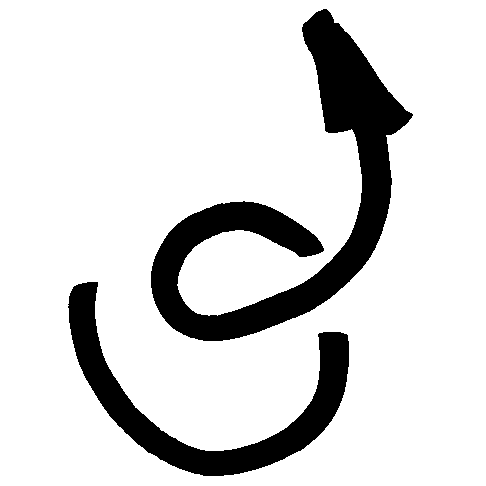
\includegraphics[totalheight=\heightof{O}]{dextro.png}}}
\newcommand*{\laevo}{\mathord{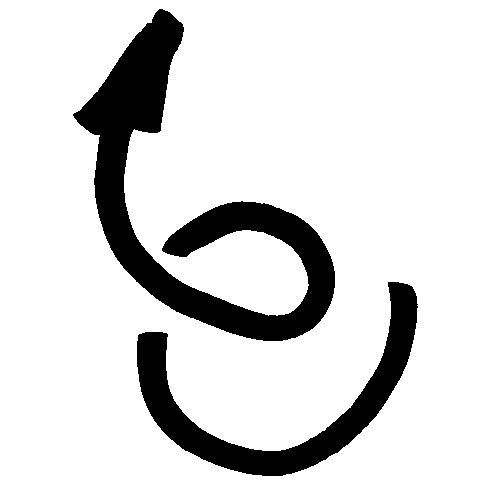
\includegraphics[totalheight=\heightof{O}]{laevo.png}}}

\definecolor{notecolour}{RGB}{68,170,153}
\newcommand*{\puzzle}{{\fontencoding{U}\fontfamily{fontawesometwo}\selectfont\symbol{225}}}
%\newcommand*{\puzzle}{\maltese}
\newcommand{\mynote}[1]{ {\color{notecolour}\puzzle\ #1}}
\newcommand*{\widebar}[1]{{\mkern1.5mu\skew{2}\overline{\mkern-1.5mu#1\mkern-1.5mu}\mkern 1.5mu}}

% \newcommand{\explanation}[4][t]{%\setlength{\tabcolsep}{-1ex}
% %\smash{
% \begin{tabular}[#1]{c}#2\\[0.5\jot]\rule{1pt}{#3}\\#4\end{tabular}}%}
% \newcommand*{\ptext}[1]{\text{\small #1}}
%\DeclareMathOperator*{\argsup}{arg\,sup}
\newcommand*{\gm}{Grassmann}
\newcommand*{\ve}{\curlyvee}
\newcommand*{\we}{\curlywedge}
\newcommand*{\co}{\centerdot}
\newcommand*{\+}{\boxplus}
\newcommand*{\yr}{r}
\newcommand*{\yN}{N}
\newcommand*{\yw}{w}
\newcommand*{\ym}{m}
\newcommand*{\ya}{a}
\newcommand*{\yb}{b}
\newcommand*{\ye}{e}
\newcommand*{\yC}{C}
\newcommand*{\yal}{\alpha}
\newcommand*{\ybe}{\beta}
\newcommand*{\ywp}{\dot{0}}
\newcommand*{\ywl}{\dot{1}}
\newcommand*{\ywa}{\dot{2}}
\newcommand*{\ywv}{\dot{3}}
\newcommand*{\zr}{\color{myred}}
\newcommand*{\zb}{\color{myblue}}
%%% Custom macros end @@@

%%%%%%%%%%%%%%%%%%%%%%%%%%%%%%%%%%%%%%%%%%%%%%%%%%%%%%%%%%%%%%%%%%%%%%%%%%%%
%%% Beginning of document
%%%%%%%%%%%%%%%%%%%%%%%%%%%%%%%%%%%%%%%%%%%%%%%%%%%%%%%%%%%%%%%%%%%%%%%%%%%%
\firmlists
\begin{document}
\captiondelim{\quad}\captionnamefont{\footnotesize}\captiontitlefont{\footnotesize}
\selectlanguage{british}\frenchspacing
\maketitle

%%%%%%%%%%%%%%%%%%%%%%%%%%%%%%%%%%%%%%%%%%%%%%%%%%%%%%%%%%%%%%%%%%%%%%%%%%%%
%%% Abstract
%%%%%%%%%%%%%%%%%%%%%%%%%%%%%%%%%%%%%%%%%%%%%%%%%%%%%%%%%%%%%%%%%%%%%%%%%%%%
\abstractrunin
\abslabeldelim{}
\renewcommand*{\abstractname}{}
\setlength{\absleftindent}{0pt}
\setlength{\absrightindent}{0pt}
\setlength{\abstitleskip}{-\absparindent}
\begin{abstract}\labelsep 0pt%
  \noindent A new view on \gm\ spaces
\\\noindent\emph{\footnotesize Note: Dear Reader
    \amp\ Peer, this manuscript is being peer-reviewed by you. Thank you.}
% \par%\\[\jot]
% \noindent
% {\footnotesize PACS: ***}\qquad%
% {\footnotesize MSC: ***}%
%\qquad{\footnotesize Keywords: ***}
\end{abstract}
\selectlanguage{british}\frenchspacing

%%%%%%%%%%%%%%%%%%%%%%%%%%%%%%%%%%%%%%%%%%%%%%%%%%%%%%%%%%%%%%%%%%%%%%%%%%%%
%%% Epigraph
%%%%%%%%%%%%%%%%%%%%%%%%%%%%%%%%%%%%%%%%%%%%%%%%%%%%%%%%%%%%%%%%%%%%%%%%%%%%
% \asudedication{\small ***}
% \vspace{\bigskipamount}
% \setlength{\epigraphwidth}{.7\columnwidth}
% %\epigraphposition{flushright}
% \epigraphtextposition{flushright}
% %\epigraphsourceposition{flushright}
% \epigraphfontsize{\footnotesize}
% \setlength{\epigraphrule}{0pt}
% %\setlength{\beforeepigraphskip}{0pt}
% %\setlength{\afterepigraphskip}{0pt}
% \epigraph{\emph{text}}{source}



%%%%%%%%%%%%%%%%%%%%%%%%%%%%%%%%%%%%%%%%%%%%%%%%%%%%%%%%%%%%%%%%%%%%%%%%%%%%
%%% BEGINNING OF MAIN TEXT
%%%%%%%%%%%%%%%%%%%%%%%%%%%%%%%%%%%%%%%%%%%%%%%%%%%%%%%%%%%%%%%%%%%%%%%%%%%%

\mynote{\footnotesize Synopsis:
  \begin{itemize}\tightlist
  \item Intro
  \item Overview
  \item Primitives (flats, weights, orientations)
  \item Sum of points with inner weight
  \item Sum of points with outer weight
  \item Sum of lines and higher-dim objects, both kinds of weight
  \item Product (join) of objects with inner weights
  \item Product (meet) of objects with outer weights
  \item Product between objects with inner and outer weights
  \item Combination of all products into a non-associative one
  \item Further discussion: non-necessity of forms etc
  \end{itemize}
}


\section{An algebra of geometric objects}
\label{sec:algebra_geometry}

The idea of a calculus analogous to \enquote{algebraic calculus, but in
  which the entities on which the calculations are carried out are
  geometric objects, instead of numbers} \citep[\chap~I, our
transl.]{peano1888} is quite old. Peano traced it back to Leibniz. He also
expressed the opinion that \enquote{before long this geometric calculus, or
  something analogous, will replace methods currently adopted in higher
  education} \citep[Prefazione, our transl.]{peano1888}.

The first consistent formulation of such a calculus is universally
attributed to \gm\ \citey{grassmann1844_r1878,grassmann1862}. Grassmann's
work was undervalued and suffered a convoluted history, an outlook of which
is given in the translator's notes of that work
\citep{grassmann1844_t1995,grassmann1862_t2000} and in the introductory
parts of several other works
\citep{peano1888,barnabeietal1985,crapo2009,browne2012,vargas2016}. His
work is surely still undervalued today. We believe part of the reason to be
the beautiful but also complicated and partially antagonist ways in which
it has been developed and presented in the past fifty years \citep[examples
are][]{hestenes1968,hestenesetal1984_r1987,barnabeietal1985,dorstetal2002,li2008,crapo2009,brinietal2011,dorstetal2011,gunn2011,browne2012,gonzalezcalvet2016,vargas2016}.
These modern presentations would probably be too difficult to digest for
high-school students.

Yet the basic ideas behind Grassmann's work are quite intuitive and easy to
visualize. They seem within the reach of a high-school student. And they
are very powerful, allowing a student to state in a couple of lines
geometric properties that would require more cumbersome formulae in
analytic geometry.


In this essay -- in the etymological sense of this term, implying
tentativeness and a want of finish -- we present an algebra of geometric
objects in the spirit of \gm\ and Peano. It differs from theirs and from
modern treatments in some mathematical respects, such as the avoidance of
metric notions and the inclusion of \enquote{exterior} and
\enquote{interior} geometric properties
\citep{veblenetal1932,schoutenetal1940,schouten1951_r1989,burke1983,burke1985_r1987,burke1995,bossavit1994_r2002,bossavit2003b}.
It also differs from modern treatments in the presentation style, which is
mainly visual, not formal, and tries to avoid advanced concepts (duals,
adjoints, matroids, and so on).



\section{Overview}
\label{sec:overview}



\section{Primitives}
\label{sec:primitives}

Our arena is three-dimensional space with its notion of \emph{parallelism}.
We won't use vectorial or metric notions such as origin, distance, or
angle; technically speaking we're considering an affine space. Denote the
dimension of space by $\yN=3$.

Our attention will focus on points, straight lines, planes, and the whole
space. By \enquote{line} we'll always mean \enquote{straight line}. When we
need to consider any one of these kinds of geometric objects, we'll call it
a \emph{flat} (for obvious reasons). When we need to keep in mind the
dimension of a flat, but the dimension is arbitrary, say $r$, we'll speak
of an \emph{$r$-flat}. Thus a point is a $0$-flat, a line a $1$-flat, and
so on.

The calculus to be introduced allows us to express geometric statements
about flats in a compact symbolic way. Some are very familiar statements of
solid geometry. For example, that a line passes through two distinct
points, or that a line is the intersection of two incident planes. Others are
statements  about relations that are not encountered in pure solid
geometry, but that we encounter in physics. For example, the statement that
a point is the centre of mass of two point-masses located at two particular
points. This second kind of statements makes our space  richer and has
consequences for the first, more familiar kind of statements.

To make the generalized kind of statements we need to enrich the geometric
objects we're considering. To each geometric object of our four basic kinds
we attribute two characteristics: a \emph{weight} and a \emph{sense}, and
each of these can be of two possible types: \emph{inner} or \emph{outer}.
For example, a point can have an inner weight and an inner sense, or
an outer weight and an outer sense; or an inner weight and an outer
sense; or, finally, an outer weight and an inner sense. A line
can also comes in those four varieties; and so on. Weight comes in
continuous degrees, whereas sense has only two possible values.

\subsection{Inner weight}
\label{sec:inner_weight}

A point with an inner weight is very akin to a point-mass in physics. The
inner weight can indeed be thought of as the mass (or charge, when combined
with an inner sense as explained below) of the point and leads to similar
statements and effects. We can freely choose a unit of mass, and it is
possible to compare the mass of any two points. The weight of a point can
thus be represented by a non-negative real number.

The inner weight of a line can be thought of as a fixed length on the line
itself.\mynote{Picture} Unlike the case of the points, a unit weight is not
defined, but it is possible to compare two possible weights of the same
line or of two parallel lines, but not of two lines that are not parallel
(incident or skew). With such comparison we can determine the ratio of the
two weights; it is a non-negative real number.\mynote{Possibly add
  discussion of how such weights are compared}\mynote{Picture}

The inner weight of a plane can be thought of as a fixed area on the plane;
but, if we visualize this area as the region within a closed curve on the
plane, we must keep in mind that the shape of such region is
unimportant.\mynote{Picture} A unit weight is not defined, but it is
possible to compare and determine the ratio of the inner weights for the
same plane or for two parallel planes, but not for two incident planes.

The inner weight of the whole space can be thought of as a fixed volume;
but, as in the case of the plane, if we visualize this volume as the region
within a closed surface we must keep in mind that the shape of such surface
is unimportant. Also in this case a unit weight is undefined but we can
compare and determine the ratio of two possible weights.\mynote{Picture}


\subsection{Inner sense}
\label{sec:inner_sense}

The inner sense of a point is simply a sign, \enquote{$+$} or
\enquote{$-$}. The combination of inner weight and inner sense can thus be
represented by a real number.

The inner sense of a line can be visualized as the direction of motion by
which we travel on the line, or of the direction of a flow happening on the
line, both familiar concepts in physics. As for inner weight, it is
possible to compare the senses of parallel lines, but not of non-parallel
ones.

The inner sense of a plane can be visualized as the direction of a circular
motion taking place on the plane. We can compare the inner senses of
parallel planes but not of non-parallel ones.

The inner sense of space (sounds funny) can be visualized as the direction
of a screw motion happening in space, again a familiar concept in physics.
We usually speak of a right-handed or dextrogyre sense,
\enquote{$\dextro$}, and of a left-handed or laevogyre sense,
\enquote{$\laevo$}.

\mynote{Pictures}

\subsection{Outer properties}
\label{sec:outer_properties}

Before introducing outer weights and senses it may be useful to help
intuition about what we mean with \enquote{outer}. Outer properties can be
visualized in several ways; we discuss two, the first more pictorial, the
second more technical.

Consider a point, and imagine to displace it a little. The freedom we have
in this displacement is three-dimensional. We can thus imagine a
three-dimensional region surrounding the point, representing its possible
displacements.

Consider a line, and imagine to displace it a little keeping it parallel to
itself. The freedom we have in this displacement is effectively
two-dimensional: two displacements that can be obtained from each other by
a displacement parallel to the line don't lead to observable differences.
We can thus imagine a two-dimensional region surrounding the line,
representing its possible effective displacements.

For a plane, the same process lead us to visualize a one dimensional region
extending on both sides of the plane.

For the space there is no effective displacement: the region to visualize
would be zero-dimensional.

The \enquote{outer region} of an $r$-flat has therefore dimension $N-r$.

\medskip

A more technical way of visualizing outer properties is in terms of
equivalence classes. For this, let's first agree to extend the meaning of
\enquote{parallel} by saying that every point is by definition parallel to
every other point.

Consider a point. The set of points parallel to (or coincident with) it is
the whole space. Let's call this the \emph{complementary space} of the point.

Consider a line, and consider the set of lines parallel to it. This set is
called the complementary space of the line. Each element of this set is a
line. The complementary space is two-dimensional. We can in fact set up a
one-to-one association between each element (a line) of this set with a
point on a plane: select a plane that intersects the original line (without
containing it in full). If we select a point on this plane, there's a
unique line parallel to the original one that passes through the chosen
point. Vice versa, if we select a line parallel to the original one, this
line passes through a unique point of the plane. Each point of this plane
is thus in one-to-one correspondence with an element of the complementary
space. Note that in this way we can associate the complementary space with
every plane that intersect the original line, so none of such planes is
preferable to the others. We can thus visualize the complementary space of
a line as a plane intersecting it, keeping in mind that the exact position
and inclination of the plane don't matter.

In an analogous way we can construct and visualize the complementary space
of a plane: it has one dimension, its elements are the planes parallel to
the original one, and it can be visualized as a line intersecting it,
keeping in mind that the exact position and inclination of such line don't
matter.

In the case of the whole space, the complementary set has just one element:
the space itself. It is therefore zero-dimensional.

The complementary space of an $r$-flat has therefore dimension $N-r$.



\subsection{Outer weights}
\label{sec:outer_weights}

Outer weights are analogous to inner weights, with the essential difference
that they are defined \emph{on the complementary space} of the point, line,
plane, or space under consideration. Since the complementary space of an
$r$-flat is $(N-r)$-dimensional, the outer weights of point, line, plane,
space are akin to the inner weights of space, plane, line, point.

A point with an outer weight can be visualized as a point with an
associated volume. We can imagine such volume as enveloping the point or
being beside it, keeping in mind that the shape and location of such volume
aren't important.

A line with an outer weight can be visualized as a line crossed by a flat
surface of given area; or as a tube, containing the original line, made of
parallel lines and having that cross-sectional area. The cross-sectional
shape of the tube doesn't matter.

A plane with an outer weight can be visualized as a plane crossed by a
segment with given length; or as two parallel planes, one on each side of
the original plane, or one of which is the original plane.

Finally, space with an outer orientation can be visualized as the whole
space with an associated non-negative number.

\mynote{Pictures}

\subsection{Outer senses}
\label{sec:outer_senses}

Outer senses are senses chosen on the complementary space of the flat under
consideration. As in the case of outer weights this leads to properties for
points, lines, planes, space that are reversed in dimensionality with
respect to inner senses.

A point with outer sense can be visualized as a point with a screw motion of
the space around it.

A line with outer sense can be visualized as a line with a rotatory motion
around it.

A plane with outer sense can be visualized as a plane with an associated
crossing direction from one side to the other.

Finally, outer sense for space is simply a sign, \enquote{$+$} or
\enquote{$-$}. The combination of outer sense and outer weight for space is
thus represented by a real number.


\mynote{Pictures}

\begin{figure}[p!]%{r}{0.4\linewidth} % with wrapfigure
 \centering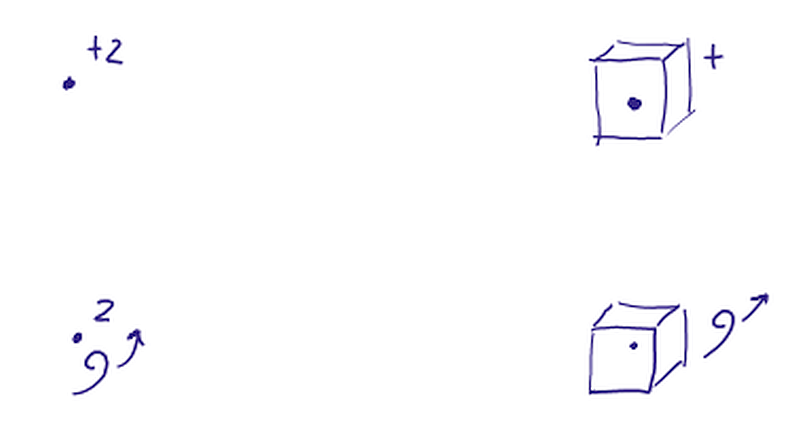
\includegraphics[width=0.9\linewidth]{ex0b.png}\\[5em]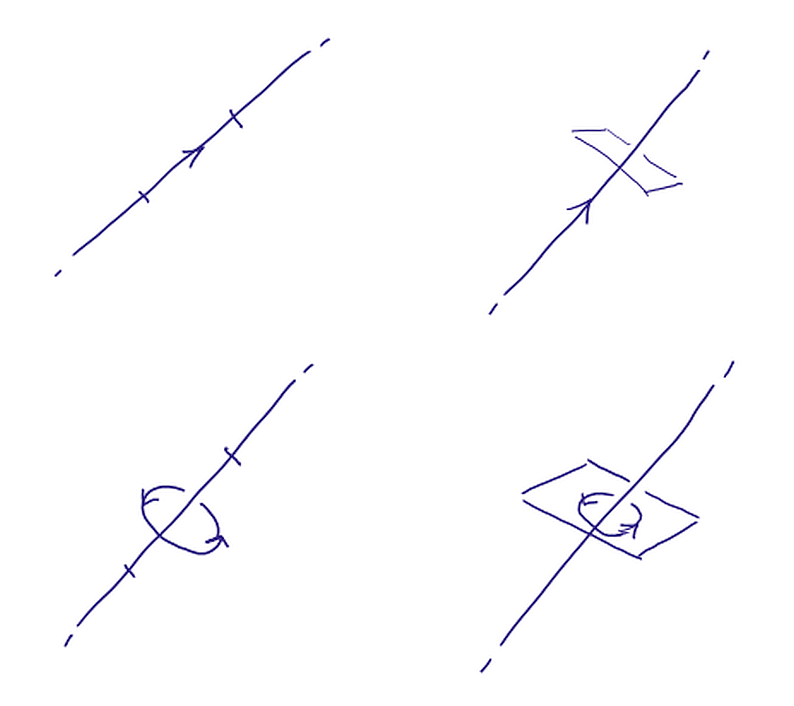
\includegraphics[width=0.9\linewidth]{ex1b.png}%
\caption{The four kinds of points and lines}\label{fig:points_lines}
\end{figure}% exp_family_maxent.nb
\begin{figure}[p!]%{r}{0.4\linewidth} % with wrapfigure
 \centering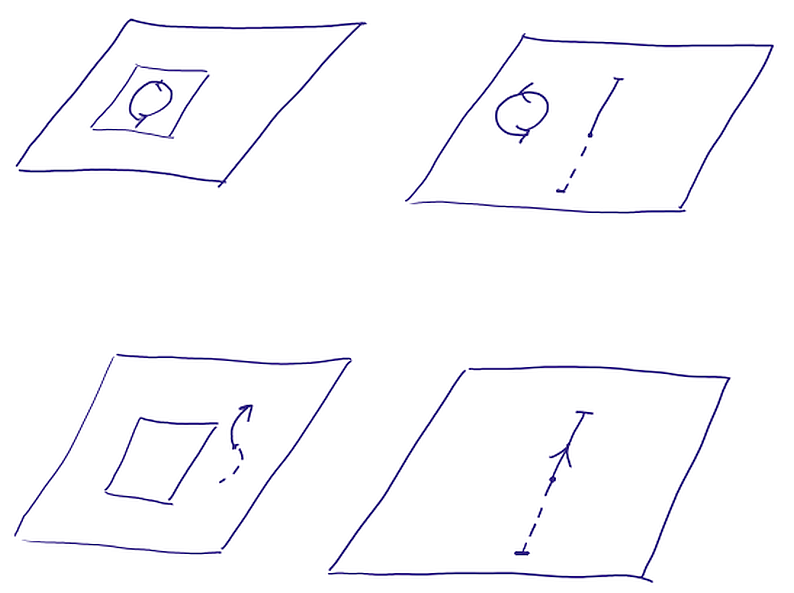
\includegraphics[width=0.9\linewidth]{ex2b.png}\\[5em]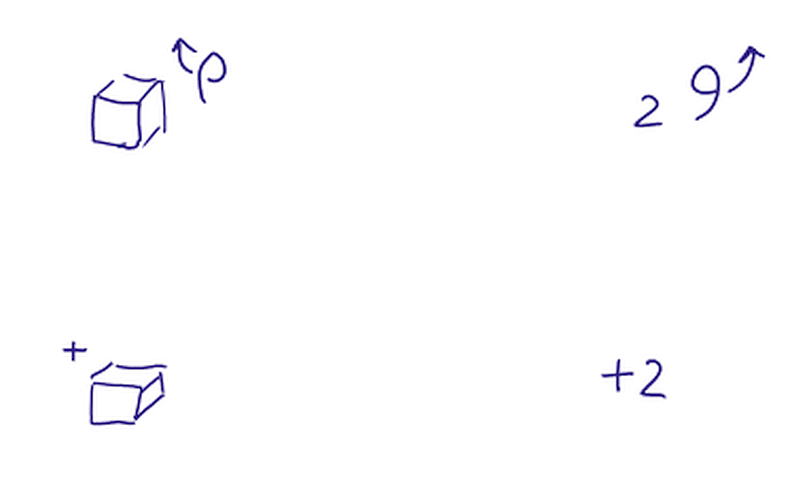
\includegraphics[width=0.9\linewidth]{ex3b.png}%
\caption{The four kinds of planes and space}\label{fig:planes_space}
\end{figure}% exp_family_maxent.nb

\subsection{Summary: zoology of geometric objects}
\label{sec:summary_kinds_objects}

Each point, line, plane, and space comes thus in four varieties:
inner-weighted and inner-oriented, outer-weighted and outer-oriented,
inner-weighted and outer-oriented, and outer-weighted and inner-oriented.
We are thus dealing with sixteen different kinds of geometrical objects.
Their visual representation is shown in
figs~\ref{fig:points_lines}--\ref{fig:planes_space}.

We have mentioned that the inner weight and inner sense of a point can be
jointly represented by a real number: its absolute value represents the
weight, its sign the sense. The same is true for the outer weight and outer
sense of space.

In the cases of a point with inner weight and outer sense, and of
space with outer weight and inner sense, the combination of weight and
sense is represented by a non-negative number with a screw sense. It is
convenient to consider negative numbers also in these cases, however: the
presence of a negative sign simply indicates that the opposite screw sense
should be considered; for example, $\dextro(-2) \equiv \laevo 2$.

The four kinds of space are especially important. Space with outer weight
and outer sense is just represented by a real number. We'll see that it has
all the properties of a \emph{scalar}, and therefore we call it that way.
Space with outer weight and inner sense behaves like a scalar with a screw
sense \citep[\cf][\sect~3.2.1]{bossavit1991}; we call it an \emph{axial
  scalar}. Space with inner weight and outer sense behaves like a
\enquote{volume element}, and we call it a \emph{pseudoscalar}. Finally, we
call space with inner weight and inner sense an \emph{axial pseudoscalar}.
Note that scalars and axial scalars have a well defined unit value, whereas
pseudoscalars of either kind don't.

We can indicate the weight of a flat independently of its sense by an
absolute-value notation, \enquote{$\abs{\dotv}$}.

\mynote{Note on Maxwell's discussion of such objects
\begin{quotation}
  Physical vector quantities may be divided into two classes, in one of
  which the quantity is defined with reference to a line, while in the
  other the quantity is defined with reference to an area. \textelp{}
  
  There is another distinction between different kinds of directed
  quantities \textelp{}. This is the distinction between longitudinal and
  rotational properties.\sourceatright{\emph{Maxwell \citey[\sects~13,
      15]{maxwell1873_r1881}}}
\end{quotation}

\begin{itemize}\tightlist
\item mass and charge density: space with inner weight and outer sense
\item current density: line with outer weight and inner sense
\item momentum density: line with outer weight and inner sense?
\item electric field: plane with outer weight and outer sense
\item magnetic field: line with outer weight and outer sense
\end{itemize}

}

\mynote{Is it best to introduce products first??}

\section{Sum of kindred objects}
\label{sec:sum_kindred}

We next show how objects in each of these sixteen categories can be
combined together to obtain an object in the same category. We assume that
the reader already has an intuitive idea of how to sum or subtract two
lengths on the same line or on two parallel lines, two areas on the same
plane or on two parallel planes, and two volumes. Remember that such sums
and subtractions do not require the notions of distance or angle.

Flats with inner weight and flats with outer weights differ in an important
respect with respect to summation. For the first, the weights generally add
up (with sign); for the second, \emph{the reciprocal of the weights}
generally add up. Thus, if we add a flat with inner
weight to itself, we obtain a flat with twice the original weight; if we
add a flat with outer weight to itself, we obtain a flat with \emph{half}
the original weight.

Let's call \emph{harmonic sum} the reciprocal of the sum of the
reciprocals, in analogy with the harmonic mean (note that this is very
different from a harmonic series), and denote it with \enquote{$\+$}.
Whereas the reciprocal of a length, area, or volume is undefined in the
absence of a notion of distance (metric), the harmonic of parallel lengths,
parallel areas, and volumes is a well-defined geometric construction even
without a notion of distance, because it can be computed in term of sums
and ratios. For example, if $\yal$ and $\ybe$ are parallel areas, their
harmonic sum is defined in terms of ratios as
\begin{equation}
  \label{eq:reciprocal_sum}
\yal \+ \ybe =  \frac{1}{\frac{1}{\yal}+ \frac{1}{\ybe}} \defd
  \frac{\ybe}{\yal+\ybe}\yal \equiv
  \frac{\yal}{\yal+\ybe}\ybe.
\end{equation}
In words, we first compute the total area $\yal+\ybe$, then the ratio
between the area $\ybe$ and this total, and finally we construct the area
that has this same ratio with the area $\yal$. \mynote{Picture} The
harmonic sum is associative just like the ordinary sum.


\subsection{Sum of points}
\label{sec:sum_points}

The sum of points with inner weight and sense generalizes the calculation
of a centre of mass and the operation of affine combination. It's
associative and commutative: it can be done in an arbitrary order.

The sum of the point $A$ with inner weight and sense $a$ and the point $B$
with inner weight and sense $b$ is a point $C$ of inner weight and sense
$a+b$, located on the line determined by $A$ and $B$, and such that the
segment with endpoints $C$, $A$ and that with endpoints $A$, $B$ are in a
ratio $\abs{b/(a+b)}$, and the segment with endpoints $B$, $C$ and that
with endpoints $A$, $B$ are in a ratio $\abs{a/(a+b)}$. A moment's thought
shows that these two requirements determine a unique location for $C$ (on
the other hand, specifying the ratio between $C,A$ and $C,B$ is not enough
to determine $C$'s position). If the ratio $b/(a+b)$ is negative, then $C$
and $B$ lie on opposite sides of $A$; analogously for the ratio $a/(a+b)$.
\mynote{Pictures}

For the sums of three non-collinear points and four mutually non-coplanar
points similar constructions exist, with the ratios referring to areas and
volumes.

\bigskip

The sum of points with inner weight and outer sense proceeds in an
analogous way, with the understanding that their screw sense behaves like a
sign, and $\dextro \equiv -\laevo$ as explained in
\sect~\ref{sec:summary_kinds_objects}.

\bigskip

The sum of the point $A$ with outer weight and inner sense $\yal$ and the
point $B$ with outer weight and inner sense $\ybe$ is a point $C$ of outer
weight and inner sense $\yal \+ \ybe$, located on the line determined by
$A$ and $B$, and such that the segment with endpoints $C$, $A$ and that
with endpoints $A$, $B$ are in a ratio $\abs{(\yal \+ \ybe)/\ybe}$, and the
segment with endpoints $B$, $C$ and that with endpoints $A$, $B$ are in a
ratio $\abs{(\yal \+ \ybe)/\yal}$. If the ratio $\abs{(\yal \+ \ybe)/\ybe}$
is negative, then $C$ and $B$ lie on opposite sides of $A$; analogously for
the other ratio. \mynote{Pictures}

\bigskip

Finally, the sum of points with outer weight and outer sense proceeds in an
analogous way as the last one, with the understanding that their screw
sense behaves like a sign, and $\dextro \equiv -\laevo$ as explained in
\sect~\ref{sec:summary_kinds_objects}.

\mynote{Find an interpretation of the sum with outer weights!}

The sums of points with outer weights may at first appear quite convoluted.
To help understand how it works it's useful to think of a point with outer
weight as a point with a unit mass that is uniformly distributed in the
volume representing to the outer weight. The outer weight itself is the
mass \emph{density} thus obtained. This explains why a doubled outer weight
is represented by a halved volume: the density is doubled, hence the unit
mass must be distributed over half the initial volume.

\section{Products}
\label{sec:products}

Let's indicate an $r$-flat with inner weight with $(\dot{r}, N-r)$ and
an $r$-flat with outer weight with $(r, \dot{N-r})$: this redundant
notation help us remember the dimensions of the flat and of its
complementary space, and of where the weight resides.

This table gives the type of flat found by multiplying flats with inner
weights -- the \emph{progressive product}:

{\centering
  \begin{tabular}{c|cccc}
    $\ve$& $(\ywp,3)$&$(\ywl,2)$&$(\ywa,1)$&$(\ywv,0)$ \\
    \midrule
    $(\ywp,3)$&$(\ywl,2)$&$(\ywa,1)$&$(\ywv,0)$& \\
    $(\ywl,2)$&$(\ywa,1)$&$(\ywv,0)$&& \\
    $(\ywa,1)$&$(\ywv,0)$&&& \\
    $(\ywv,0)$&&&& 
  \end{tabular}

}
the empty entries being zero.

This table gives the type of flat found by multiplying flats with outer
weights -- the \emph{regressive product}:

{\centering
  \begin{tabular}{c|cccc}
    $\we$& $(0,\ywv)$&$(1,\ywa)$&$(2,\ywl)$&$(3,\ywp)$ \\
    \midrule
    $(0,\ywv)$&&&&$(0,\ywv)$ \\
    $(1,\ywa)$&&&$(0,\ywv)$&$(1,\ywa)$ \\
    $(2,\ywl)$&&$(0,\ywv)$&$(1,\ywa)$&$(2,\ywl)$ \\
    $(3,\ywp)$&$(0,\ywv)$&$(1,\ywa)$&$(2,\ywl)$&$(3,\ywp)$ \\
  \end{tabular}

}
the empty entries being zero.
        
This table gives the type of flat found by multiplying flats with inner
weights and flats with outer weights -- the \emph{contraction}:

{\centering
  \begin{tabular}{c|cccc}
    $\co$& $(0,\ywv)$&$(1,\ywa)$&$(2,\ywl)$&$(3,\ywp)$ \\
    \midrule
    $(\ywp,3)$&$(1,\ywa)$&$(2,\ywl)$&$(3,\ywp)$&$(\ywp,3)$ \\
    $(\ywl,2)$&$(2,\ywl)$&$(3,\ywp)$&$(\ywp,3)$&$(\ywl,2)$ \\
    $(\ywa,1)$&$(3,\ywp)$&$(\ywp,3)$&$(\ywl,2)$&$(\ywa,1)$ \\
    $(\ywv,0)$&$(\ywp,3)$&$(\ywl,2)$&$(\ywa,1)$&$(\ywv,0)$ \\
  \end{tabular}

}

\bigskip

From the last two tables we see that a space with outer weight, type
$(3,\ywp)$, behaves like a scalar. Moreover, the general structure of the
three tables suggest that we could complete the first two in the following
way:

{\centering
  \begin{tabular}{c|cccc}
    & $(\ywp,3)$&$(\ywl,2)$&$(\ywa,1)$&$(\ywv,0)$ \\
    \midrule
    $(\ywp,3)$&$(\ywl,2)$&$(\ywa,1)$&$(\ywv,0)$&$(0,\ywv)$ \\
    $(\ywl,2)$&$(\ywa,1)$&$(\ywv,0)$&$(0,\ywv)$&$(1,\ywa)$ \\
    $(\ywa,1)$&$(\ywv,0)$&$(0,\ywv)$&$(1,\ywa)$&$(2,\ywl)$ \\
    $(\ywv,0)$&$(0,\ywv)$&$(1,\ywa)$&$(2,\ywl)$&$(3,\ywp)$ \\
  \end{tabular}

}

\bigskip
{\centering
  \begin{tabular}{c|cccc}
    & $(0,\ywv)$&$(1,\ywa)$&$(2,\ywl)$&$(3,\ywp)$ \\
    \midrule
    $(0,\ywv)$&$(\ywl,2)$&$(\ywa,1)$&$(\ywv,0)$&$(0,\ywv)$ \\
    $(1,\ywa)$&$(\ywa,1)$&$(\ywv,0)$&$(0,\ywv)$&$(1,\ywa)$ \\
    $(2,\ywl)$&$(\ywv,0)$&$(0,\ywv)$&$(1,\ywa)$&$(2,\ywl)$ \\
    $(3,\ywp)$&$(0,\ywv)$&$(1,\ywa)$&$(2,\ywl)$&$(3,\ywp)$ \\
  \end{tabular}

}

On the other hand we can consider the table for the contraction as really
an extension of progressive (above the anti-diagonal) and regressive
(anti-diagonal and below) products. Likewise, the new parts in the last two
tables extend the regressive and progressive products. This way we are left
with two products with the following tables:

\bigskip

{\centering
  \begin{tabular}{c|ccccccccc}
    $\ve$& $(\ywp,3)$&$(\ywl,2)$&$(\ywa,1)$&$(\ywv,0)$  &
 &$(0,\ywv)$&$(1,\ywa)$&$(2,\ywl)$&$(3,\ywp)$ \\
    \midrule
    $(\ywp,3)$&$(\ywl,2)$&$(\ywa,1)$&$(\ywv,0)$&&
 &$(1,\ywa)$&$(2,\ywl)$&$(3,\ywp)$& \\
    $(\ywl,2)$&$(\ywa,1)$&$(\ywv,0)$&&&
 &$(2,\ywl)$&$(3,\ywp)$&& \\
    $(\ywa,1)$&$(\ywv,0)$&&&&
 &$(3,\ywp)$&&& \\
    $(\ywv,0)$&&&&&
 &&&& \\
 &&&&&&&&& \\
    $(0,\ywv)$ &$(1,\ywa)$&$(2,\ywl)$&$(3,\ywp)$&&
 &$(\ywl,2)$&$(\ywa,1)$&$(\ywv,0)$& \\                                         
    $(1,\ywa)$ &$(2,\ywl)$&$(3,\ywp)$&&&
 &$(\ywa,1)$&$(\ywv,0)$&& \\                    
    $(2,\ywl)$&$(3,\ywp)$&&&&
 &$(\ywv,0)$&&& \\
 $(3,\ywp)$&&&&&&&&& 
  \end{tabular}

}
empty entries being zero.

\bigskip

{\centering
  \begin{tabular}{c|ccccccccc}
    $\we$& $(\ywp,3)$&$(\ywl,2)$&$(\ywa,1)$&$(\ywv,0)$  &
 &$(0,\ywv)$&$(1,\ywa)$&$(2,\ywl)$&$(3,\ywp)$ \\
    \midrule
    $(\ywp,3)$&&&&$(0,\ywv)$ &
     &&&&$(\ywp,3)$ \\
    $(\ywl,2)$&&&$(0,\ywv)$&$(1,\ywa)$ &
&&&$(\ywp,3)$&$(\ywl,2)$ \\
    $(\ywa,1)$&&$(0,\ywv)$&$(1,\ywa)$&$(2,\ywl)$ &
&&$(\ywp,3)$&$(\ywl,2)$&$(\ywa,1)$ \\
    $(\ywv,0)$&$(0,\ywv)$&$(1,\ywa)$&$(2,\ywl)$&$(3,\ywp)$ &
 &$(\ywp,3)$&$(\ywl,2)$&$(\ywa,1)$&$(\ywv,0)$ \\
 &&&&&&&&& \\
    $(0,\ywv)$&&&&$(\ywp,3)$ &
&&&&$(0,\ywv)$ \\                               
$(1,\ywa)$&&&$(\ywp,3)$&$(\ywl,2)$ &
&&&$(0,\ywv)$&$(1,\ywa)$ \\
 $(2,\ywl)$&&$(\ywp,3)$&$(\ywl,2)$&$(\ywa,1)$ &
 &&$(0,\ywv)$&$(1,\ywa)$&$(2,\ywl)$ \\
 $(3,\ywp)$&$(\ywp,3)$&$(\ywl,2)$&$(\ywa,1)$&$(\ywv,0)$ &
 &$(0,\ywv)$&$(1,\ywa)$&$(2,\ywl)$&$(3,\ywp)$
  \end{tabular}

}
empty entries being zero.

\bigskip

Note the following relations regarding weights, similar to the
multiplication of signs:
\begin{equation}
  \label{eq:parities_products}
  \begin{aligned}
    \text{inner}\ve\text{inner}&=\text{inner}
    &\qquad
      \text{inner}\we\text{inner}&=\text{outer}
\\
    \text{outer}\ve\text{outer}&=\text{inner}
    &\qquad
    \text{outer}\we\text{outer}&=\text{outer}
    \\
    \text{inner}\ve\text{outer}&=\text{outer}
&\qquad
    \text{inner}\we\text{outer}&=\text{inner}
  \end{aligned}
\end{equation}

This is the table for the meet, join, and contraction:

{\centering
  \begin{tabular}{c|cccc|cccc}
    $\zb\ve$ $\zr\we$ $\cdot$&$0$&$1$&$2$&$3$ 
& $\ywp$&$\ywl$&$\ywa$&$\ywv$  \\
    \midrule
$0$& &&$\ywv$&$0$
&$\zb1$&$\zb2$&$3$&$\ywp$ \\
$1$&&$\ywv$&$\zr0$&$1$ 
&$\zb2$&$3$&$\zr\ywp$&$\ywl$ \\
$2$&$\ywv$&$\zr0$&$\zr1$&$2$ 
&$3$&$\zr\ywp$&$\zr\ywl$&$\ywa$ \\
 $3$&$0$&$1$&$2$&$3$ 
&$\ywp$&$\ywl$&$\ywa$&$\ywv$ \\
%    
 $\ywp$&$\zb1$&$\zb2$&$3$&$\ywp$
&$\zb\ywl$&$\zb\ywa$&$\ywv$&\\
 $\ywl$&$\zb2$&$3$&$\zr\ywp$&$\ywl$
&$\zb\ywa$&$\ywv$&&\\
 $\ywa$&$3$&$\zr\ywp$&$\zr\ywl$&$\ywa$
&$\ywv$&&&\\
 $\ywv$&$\ywp$ &$\ywl$&$\ywa$&$\ywv$
&&&&
  \end{tabular}

}
empty entries being zero.

\bigskip


\bigskip\mynote{The question whether we can  replace the zero entries of the first
  two tables pivots around this problem:

  Consider five points with inner weight: $A_1,\dotsc,A_5$. The fact that
  all of them lie in the same space can be expressed with the progressive
  product as $A_1 \ve\dotsb\ve A_5 = 0$. The regressive product of the
  space $A_1 \ve\dotsb\ve A_4$ and the point $A_5$ is instead non-zero:
  $(A_1 \ve\dotsb\ve A_4) \we A_5 \ne 0$. There is no way to make allowance for
  both these statements with one product only, even if non-associative.}

\clearpage
\hrule
OLD TEXT
\hrule
\bigskip

\subsection{$\yr$-flats}
\label{sec:flats}

$\yr$-dimensional \emph{flats} or $\yr$-flats: a 1-flat is a straight line,
a 2-flat a plane, the 3-flat is the whole space, and a 0-flat is a point.
Two flats can be parallel, incident, or skew \mynote{example pictures}.
Every $\yr$-flat is itself an affine space of $\yr$ dimensions.

\subsection{$\yr$-coflats}
\label{sec:coflats}

An $\yr$-dimensional \emph{co-flat} or $\yr$-coflat, is the set of
$\yr$-flats parallel to a given $\yr$-flat. For example, given a straight
line, the set of lines parallel to it is a 1-flat. Every $\yr$-coflat is
itself an affine space of $\yN-\yr$ dimensions. Every $\yr$-flat determines
a unique $\yr$-coflat, but not vice versa.

We can always set up a non-canonical identification between an $\yr$-coflat
and an $(\yN-\yr)$-flat. Consider for example a line. The set of lines
parallel to it constitutes a 1-coflat or co-line. Select a plane that
intersects this line without containing it. Each line parallel to the given
one passes through one point of this plane, in a one-one correspondence.
The points of this plane thus correspond to the points of the 1-coflat
determined by the given line. Every plane that intersect the original line
has this isomorphism with the 1-coflat; this is why this identification is
non-canonical. In a similar fashion, if we select a plane, the set of
planes parallel to it constitute a 2-coflat or co-plane. This set is an
affine space of 1 dimension. Choose a line intersecting the original plane
in one point. Each point on this line selects a unique plane parallel to
the original one, and thus selects one point on the 2-coflat.


\subsection{$\yr$-extensions}
\label{sec:extensions}

Given an $\yr$-flat, we can select a $\yr$-dimensional region of it (not
necessarily simply connected) delimited by a closed $(\yr-1)$-dimensional
manifold. For example, a 2-dimensional region bounded by closed curve on a
plane \mynote{add example pictures}. The absence of a metric doesn't allow
us to speak of the exact extension of this region -- its length, or area,
or volume. But parallelism allows us to give a numerical value to the
\emph{ratio} of the extensions of two different regions on the same
$\yr$-flat or on parallel $\yr$-flats. In particular, it allows us to say
whether two such regions have the same extension. An $\yr$-extension is the
equivalence class of the regions having the same extension. It can be
visualized as a region on an $\yr$-flat, but the location and shape of this
region don't matter, as long as we preserve its extension.

We define a 0-extension as a positive real number.

\mynote{Pictures}

\subsection{$\yr$-coextensions}
\label{sec:coextensions}


Now consider an $\yr$-coflat. It's an affine space, so we can consider an
$(\yN-\yr)$-dimensional region on it and an $(\yN-\yr)$-extension. This is
called an $\yr$-coextension.

Coextensions can be visualized in two ways. Consider a 1-coextension. We
select a line, and this determines a co-line. We can visualize this co-line
as a plane intersecting the original line. A 1-coextension is visualized as
a closed 2-dimensional region on this plane, with the understanding that
its location and shape don't matter, as long as its area is the same. Thus
a 1-coextension can be identified with a 2-dimensional flat region
intersecting a given line \mynote{picture}. On the other hand, consider the
abstract 2-dimensional region in the co-line. This region has a boundary;
the points of this boundary represent lines parallel to the original one.
We can thus visualize a 1-coextension as a tube formed by parallel lines,
with the understanding that the cross-sectional shape of the tube doesn't
matter, as long as its cross-sectional area with respect to any plane
cutting it, remains the same.

Proceeding in a similar way, we can visualize:
\begin{itemize}
\item a 2-coextension as a segment on a line intersecting a given plane, or
  as two parallel planes;
\item a 0-coextension as a 3-dimensional region of space, with the
  understanding that its shape and location don't matter, as long as its
  volume is the same;
\item a 3-coextension is defined as a positive real number.
\end{itemize}

\mynote{Pictures}

\subsection{Orientations}
\label{sec:orientations}






Our primitive objects are point, line, plane, space. But we equip each of
these with two characteristics: a \emph{weight} and an \emph{orientation}. Weight
and orientation can each be of two kinds: \emph{inner}, that is, defined on the
geometric object itself; or of \emph{outer} kind, that is, defined on the
complement subspace of the object.



\clearpage
\hrule
OLD TEXT
\hrule
\bigskip
{\footnotesize\mynote{IMPORTANT: several statements below are \emph{false}
    and will be corrected later. This happens because they  concern
    notions at the \enquote{boundaries} of the references given in the
    first section, which aren't developed in any of those works. For
    example, statements about the scalar multiplication of outer-weighted
    objects. I'm working this out.}}

\mynote{Most important todo:
  \begin{itemize}
  \item clarify if and how Whitney forms and \enquote{elements} fit into
    \gm\ algebra.
  \end{itemize}
}

\mynote{Other refs to check:  \cite{barnabeietal1985,crapo2009,brinietal2011,bossavit1999_r2004,whitney1957,bossavit2002_r2005,arnoldetal2006,sternetal2015}}

\section{Why}
\label{sec:why}

These notes present \gm\ spaces by combining \gm's ideas as summarized by
Peano \citey{peano1888}, ideas from geometric algebra
\cite{dorstetal2007,li2008}, the concept of outer-oriented or
\enquote{twisted} geometric objects
\cite{veblenetal1932,schoutenetal1940,schouten1951_r1989,burke1983,burke1985_r1987,burke1995,bossavit1994_r2002,bossavit2003b},
the theory of Whitney elements introduced by Bossavit
\cite{bossavit2002_r2005,bossavit2003b,whitney1957,gawliketal2010,brinietal2011,arnoldetal2009_r2010}
% de Rham cohomology \cite{derham1955_t1984,arnoldetal2009_r2010},
and insights from Barnabei, Brini, Rota's
\citey{brinietal2011,barnabeietal1985}, Goldman's
\citey{goldman2002,goldman2000}, and Crapo's \citey{crapo2009} brilliant
presentations. \mynote{add also
  \cite{bambergetal1988_r1990,bambergetal1990_r1992,frankel1997_r2012}}

These notes do not contain anything new, except maybe the glue joining the
works above. We will rest content if we manage to spark your curiosity and
to spur you to take a look at them.

\textcolor{white}{If you find this you can claim a postcard from me.}

\gm\ spaces are beautiful. They share many important properties with
projective spaces, yet are as intuitive as affine spaces. They represent
notions like point, vector, functional, form on an equal geometric level.
Their geometric operations have a beautiful algebra and include a
simplified version of the operations of of integration, differentiation,
boundary and the de~Rham theory of chains and cochains on manifolds. Their
geometric notions can be given intuitive physical interpretations and be
computationally used for the numerical solution of partial
integro-differential equations. \mynote{Maybe add something about their
  relation to Cayley algebras}

The primitives of \gm\ spaces are the same as for affine spaces: point,
straight line, plane, and so on; and the notion of parallelism. But each of
these geometric objects has also a \emph{weight density} and an
\emph{orientation}. Weight and orientation can be of \emph{inner} kind,
that is, defined on the geometric object itself; or of \emph{outer} kind,
that is, defined on the complement subspace of the object.


\section{Basic geometric objects and properties}
\label{sec:basic_objects_properties}


\subsection{Basic geometric objects}
\label{sec:points_etc}

The basic geometric objects of a \gm\ space are those of an affine space:
points, straight lines, planes, and so on. We assume these are well-known
to you. Let's agree to use the terms \emph{point}, \emph{line},
\emph{plane} with their usual $0$-, $1$-, $2$-dimensional meanings. We call
\emph{$\yr$-plane} their $\yr$-dimensional generalization, a $0$-plane
being a point, and so on. In a space of dimension $\yN$ we call
\emph{hyperplane} an $(\yN-1)$-plane; there is only one $\yN$-plane, the
space itself.

The notion of parallelism is very important, and we assume that it is also
well-known to you. Just like in an affine space, there is no notion of
angle or orthogonality, nor is there an absolute measure of length, area,
and so on. We want to remind that the notion of parallelism, though, allows
us to meaningfully speak of the ratio of lengths of segments lying on
parallel lines, the ratio of areas lying on parallel planes, and so on.

Important: a weight density, to be introduced shortly, is \emph{not} the
same as a relative length, area, \etc, although these notions are related.

\subsection{Complements}
\label{sec:complements}

The notion of \emph{complement} is essential. Let's explain it in detail,
starting with an example.

Consider a line in a 3-dimensional space. We can consider the set of this
line and all lines parallel to it, see \fig\mynote{}. The \enquote{points} of
this set are the parallel lines of our original space. This set is
2-dimensional and has an affine structure and a notion of parallelism. For
example, two parallel lines in this set correspond to two parallel planes
containing some of the parallel lines our set is made of. This set is
called the \emph{complement} of our line.

If we select a plane intersecting our line in only one point, then there is
a one-one correspondence between it and the complement. For example, a
point on the plane corresponds to the unique line parallel to our initial
one and passing through this point, and vice versa; and this line is a
\enquote{point} in the complement. We can therefore speak of objects,
properties, constructions on the complement of our line by referring to a
specific plane intersecting this line -- remembering, though, that such
properties are not specific to that plane but shared by all other planes
intersecting this line.

Generalizing to an $\yr$-plane in an $\yN$-dimensional space, its
complement is $(\yN-\yr)$-dimensional and is in one-one correspondence with
each $(\yN-\yr)$-plane intersecting the original $\yr$-plane in only one
point.

Two parallel $\yr$-planes have the same complement. The complement of a
point is isomorphic to the whole space, and the complement of the whole
space is in one-one correspondence with each point.


%\subsection{Weight densities and orientations, inner and outer}
%\label{sec:weights_orientations}


\subsection{Weight densities}
\label{sec:weight_densities}

With each $\yr$-plane we can associate a \emph{weight density}, or simply
\enquote{weight}, represented by a non-negative real number. Of a point we
simply say that it has a weight.

Assigning a weight to an $\yr$-plane is different from assigning a unit
length to it, although the two notions are related. Consider for example
the two parallel lines of \fig\mynote{}. The first has a total weight $\yw$
associated with the segment $AB$, the second a total weight $2\yw$
associated with the segment $CD$, which has twice the length of $AB$. The two
parallel lines have therefore the same weight density.

It is therefore only meaningful to compare the weight densities of parallel
$\yr$-planes.


\subsection{Orientations}
\label{sec:orientations2}

It is easy to familiarize with the notion of orientation of a line, plane,
volume. We can imagine to traverse a line with two points $A$, $B$ by going
from $A$ to $B$ or from $B$ to $A$. On a plane we can imagine to
\enquote{spin} clockwise or counter-clockwise. In a volume we can identify
two cork-screw senses. In each case there are two possible orientations. In
the $0$-dimensional case of a point we convene to have the two symbolic
orientations \enquote{$+$} and \enquote{$-$}. 

Mathematically orientation is usually defined in terms of some equivalence
class. This shows that, as with all notions defined in terms of equivalence
classes, the mathematical formalism is still too primitive to capture it
well. In this note we would like to consider orientation as intuitive and
primitive, and will try not to use equivalence classes to define it.

The choice of an orientation on a line determines a unique ordering of
every two distinct points on it. The choice of an orientation on a plane
determines a unique ordering of every three non-collinear points on it,
modulo an even number of permutations in the ordering. And so on for
$\yr$-planes.

If a particular orientation is understood on a set of $\yr$-planes, we can
understand a negative weight as indicating a reversed orientation. This
corresponds to multiplying the positive weight by $-1$, as explained below.


\subsection{Inner and outer properties}
\label{sec:inner_outer_properties}

Weight and orientation were defined above as \enquote{lying} within an
$\yr$-plane. For this reason they are called \emph{inner}, and we say that
an $\yr$-plane has an inner weight or is inner-oriented.

Now consider the complement of an $\yr$-plane in an $\yN$-dimensional
space. This is an $(\yN-\yr)$-dimensional affine space, and also the unique
$(\yN-\yr)$-plane within this space. We can associate with it a weight and an
orientation. As it happens with all properties defined on a complement, they
can be mapped one-to-one onto every $(\yN-\yr)$-plane intersecting the
initial $\yr$-plane in our original space; each such $(\yN-\yr)$-plane
therefore acquires a weight and an orientation. Vice versa we can
speak of the weight and orientation of a complement by referring to any
$(\yN-\yr)$-plane intersecting our initial $\yr$-plane.

When we assign a weight $\yw$ to the complement of an $\yr$-plane, we say
that the latter has an \emph{outer} weight $1/\yw$ -- note the reciprocal.
When we assign an orientation to the complement, we say that the
$\yr$-plane has an \emph{outer} orientation.

Inner and outer weights and orientations can be assigned independently of
each other. Given an $\yr$-plane we have therefore four possibilities: we
can assign to it an inner weight and inner orientation, an outer weight and
outer orientation, an inner weight and outer orientation, an outer weight
and inner orientation. \mynote{Can we also assign all four?}

Let's see the special case of points in 2-dimensional space, \ie\ a plane;
see \fig\mynote{}. A point with inner weight and inner orientation simply
has an associated real number, positive or negative. A point with outer
weight $\ym$ and outer orientation assigns a weight surface density $1/\ym$
and a circulation sense to the whole plane. A point with inner weight and
outer orientation has an associated positive real number and a circulation
for the plane; a negative real number indicates that the opposite
circulation must be taken. Finally, a point with outer weight $\ym$ and
inner orientation assigns a weight surface density $1/\ym$ to the whole
plane and has an associated $+$ or $-$ sign; a negative density indicates
that the opposite sign must be taken.

The case of a line in 3-dimensional space is illustrated in \fig\mynote{}.


\section{Scalar multiplication and sum}
\label{sec:multiplication_sum}

We indicate weighted and oriented $\yr$-planes simply by their weights, if
this does not cause confusion. A negative weight means an opposite
orientation with respect to a tacitly understood one.

Each $\yr$-plane with a weight and orientation, either inner or outer, can
be multiplied by a real number. The result is the same $\yr$-plane with its
weight multiplied by the absolute value of the number, and the same or a
reversed orientation depending on whether the number is positive or
negative. See \fig\mynote{}

Two $\yr$-planes, both having inner or outer properties, can also be
summed. 

Let's start with the sum of weighted points, $\ym_1$, $\ym_2$, \ldots. This
is an interesting operation because it generalizes affine combination and
leads to properties alike those of projective space.

First assume that the sum of the weights does not vanish:
$\sum_j\ym_j \ne 0$. The result of the sum of the weighted points is a
point given by the usual affine combination of the points with normalized
coefficients $\ym_i/\sum_j\ym_j$, and with an associated weight
$\sum_j\ym_j$. \mynote{Add definition or example of affine combination}.
The resulting weight and orientation are inner or outer depending on
whether those of all the summand points are.

Now consider the case of vanishing total weight, and for simplicity
consider just two points: $\ym_1 + \ym_2 = 0$. By writing $\ym_2 = \epsilon
-\ym_1$ and considering smaller and smaller values of $\epsilon$, we see
that the resulting point is \enquote{at infinity} and has a vanishing
weight; its orientation is therefore also undetermined.

Points of this kind are called \emph{vectors}. They have indeed all
properties of usual \enquote{free vectors}. Consider for example two points
$A$, $B$ with unit weights and positive orientation, and the vector
$v \defd B-A$. By summing this vector to the point $A$ we obtain the point
$B$: $A+v = B$. Thus $v$ really behaves as a vector from $A$ to $B$,
translating the point $A$ to $B$ when summed to the former.

Vectors also give \gm\ spaces properties typical of projective spaces.
Consider for example the unit-weight points $A$, $B$ on the line $\ya$, and
two unit-weight points $C$, $D$ on the parallel line $\yb$ and having the
same distance as $A$, $B$. The vectors $B-A$ and $D-C$ are the same. This
can be seen by rewriting the equality $B-A = D-C$ as $A+D = B+C$, which is
indeed satisfied because the result of both $A+D$ and $B+C$ is the point at
the centre of their parallelogram, with a weight of $2$. This means that
the vector $B-A$ is a point belonging to both parallel lines $\ya$ and
$\yb$, which therefore \enquote{meet at infinity}. A vector therefore
characterizes the common direction, or \emph{attitude}, and inner
orientation of a set of parallel lines.

But the presence of weights leads to a much richer and interesting
structure than in affine and projective spaces. Consider for example the
vector $v \defd B-A$, and sum it to the point $A$ having a large weight
$\ym$, which we denote $\ym A$. The result is the point $B+(\ym-1)A$,
located at relative distances $(\ym-1)/\ym$ from $B$ and $1/\ym$ from $A$.
As the weight $\ym$ increases, this resultant point gets closer to $A$.
Thus the amount by which a weighted point is translated by a vector depends
on the point's weight, a \enquote{heavy} point being translated less than a
\enquote{light} one.

For an exploration of these fascinating properties and their use we
recommend Goldman's brilliant articles \cite{goldman2000,goldman2002}.

\mynote{Explore and add more curiosities of this kind}


\medskip

Above we spoke of the total sum of the weights of some points, implicitly
assuming that these weights can somehow be summed independently of the
points they belong to. This is possible because all points have the same
complement -- the whole space -- or equivalently because they are all
\enquote{parallel} to one another.

The weights of parallel $\yr$-planes can similarly be added, taking care of
their orientations, independently of the $\yr$-planes they belong to. The
reason is exactly the same as for the comparison of lengths, surfaces,
\etc, of parallel objects in an affine space.

Sums of parallel $\yr$-planes with total zero weight are objects called
$\yr$-vectors, analogous to vectors. They can be imagined as $\yr$-planes
\enquote{at infinity} with vanishing weight. An $\yr$-vector is
\enquote{common} to a set of parallel $(\yr+1)$-planes, and therefore
characterizes their $\yr$-direction or attitude and inner orientation.
Again this gives many projective-like properties to a \gm\ space.

\mynote{The following example needs the introduction of wedge first} Let's
consider the two-dimensional case of \emph{bivectors}. Consider the
antiparallel lines $A\we B$ and $-C\we D$, the distances $AB$ and $CD$
being equal. The total weight of these lines is zero. The sum
$A \we B - C \we D$ is a bivector. It can be considered as a
\enquote{line} that \enquote{goes around} the plane containing $A \we B$
and $C \we D$, with a circulation sense agreeing with those of $AB$ and
$CD$. See \fig\mynote{}.

The segment $CD$ is parallel to $AB$, hence there is a vector $w$ such that
$C = A + w$ and $D = B + w$. The bivector
$\yal \defd A \we B - C \we D$ is therefore equal to $(B-A) \we w$,
or $\yal = v \we w$, with $v \defd B-A$. A bivector is therefore equal to
the product of two vectors.

Very interesting is the case of $\yr$-planes that are skew, that is, do not
lie on a common $(\yr+1)$-plane. Their weights cannot meaningfully be
summed. ***


\mynote{Explain sum of lines and planes with examples}

The literature uses the term \emph{extensors} to indicate points, lines,
\etc\ that can be both of the usual kind and \enquote{at infinity},
reserving \enquote{point} \etc\ only for those not at infinity.
\mynote{Shall we also use it?}

\section{Join, meet, contraction}
\label{sec:join_meet_contraction}

Besides sum and scalar multiplication, \gm\ spaces have three kinds of
multiplicative operations: join, meet, and contraction.

The join  operates on inner-weighted objects, giving a new inner-weighted
object of higher dimension. The meet  operates on outer-weighted
objects, giving a new outer-weighted object of lower dimension, hence
higher codimension. 


\subsection{Wedge or join} 
\label{sec:wedge} 

The common notion of vector is usually associated with a line, but we have seen
that vectors in \gm\ spaces are special kinds of points, and indeed they
have properties more similar to points than lines.

A line with inner weight and orientation also has many similarities to a
vector. The main difference is that it is not a free vector, because it is
bound to that particular line; but it is not a bound vector either, because
it has no definite initial point within that line.

\mynote{Not sure whether the paragraphs above are understandable}

\gm\ spaces have also another operation, the \emph{wedge product}, which
yields \emph{inner-weighted} objects of higher dimension from
lower-dimensional ones.

Let's start with two inner-weighted, inner-oriented points $\ym_1$,
$\ym_2$. The result of their wedge product $\ym_1 \we \ym_2$ is the line
passing through them, having weight $\ym_1\ym_2$ and inner orientation
going from the first to the second; if the total weight is negative then
the opposite orientation must be taken. See \fig\mynote{}.


\mynote{Clarify the difference between \enquote{wedge} and \enquote{join}
  in the literature}

The wedge product of \emph{outer-weighted} objects yields a
lower-dimensional object instead.\mynote{That's why Barnabei, Brini, Rota
  \cite{barnabeietal1985,brinietal2011} indicate the wedge of
  inner-weighted objects with $\lor$ and that of outer-weighted ones with
  $\land$, reminding of $\cup$ and $\cap$.}


\medskip


Consider the exterior algebra of a 4-dimensional vector space, with four
linearly independent vectors $\ye_1$, $\ye_2$, $\ye_3$, $\ye_4$. The
products $\ye_1\we\ye_2$ and $\ye_3\we\ye_4$ can be associated with two
planes containing the respective vectors. These planes  intersect at one
point only, the origin. It is for this reason that the sum $\ye_1\we\ye_2
+ \ye_3\we\ye_4$ cannot be written as $a \we b$.

% This does not happen for the wedge product of a \gm\ space. Consider four
% non-coplanar points $A_1$, $A_2$, $A_3$, $A_4$. We have $A_1\we A_2 +
% A_2\we A_3 + A_3\we A_4 + A_4\we A_1 = 0$, which implies $A_1 \we
% A_2 + A_3 \we A_4 = A_1 \we A_4 + A_3 \we A_2$. Now consider the
% midpoints $B$ between $A_1$ and $A_3$,  $B \defd (A_1 + A_3)/2$, and $C$
% between $A_2$ and $A_4$, $C \defd (A_2 + A_4)/2$. Their product, given the
% equality just proven, is
% \begin{equation}
%   \label{eq:ABCDisEF}
%   \begin{split}
%     B \we C &= (A_1 \we A_2 + A_3\we A_4)/4 +
%     (A_1 \we A_4 + A_3\we A_2)/4,\\
%     &= (A_1 \we A_2 + A_3\we A_4)/2.
%   \end{split}
% \end{equation}
% A sum of weighted lines of the form $A_1 \we A_2 + A_3 \we A_4$ can therefore be
% interpreted as a weighted line: $2 B \we C$.



\section{Contraction or meet}
\label{sec:contraction}

\mynote{There are two main approaches around:
  \begin{itemize}
  \item The \enquote{geometric-algebra school} introduce a metric and a
    dual space, and define the meet in terms of contractions with duals and
    scalar products. Whitney seems to do likewise, at least at the
    beginning of his book.
  \item The \enquote{Rota school} introduce a volume element
    ($\yN$-covector) and define the meet in terms of the latter. Their
    approach is to view a \emph{Peano space} in terms of invariance under
    the special linear group -- that is, the preservation of volumes.
  \end{itemize}
  Neither school introduce a distinction between inner- and outer-weighted
  objects. Barnabei, Brini, \amp\ Rota make one valid observation:
  \begin{quote}\small
    Elie Cartan found the regressive product to be superfluous and awkward.
    By vector space duality, a pairing of the two exterior algebras of $V$
    and $V^*$ could easily be made with only one kind of product, the one
    that came to be called the wedge. \textelp{However, T}he dual space
    $V^*$ of a vector space $V$ plays no role in such a calculus: a
    hyperplane is an object living in $V$, and its identification with a
    linear functional is a step backwards in clarity.
  \end{quote}
  I think that their geometric viewpoint would be even more elegant by
  distinguishing between inner and outer weights. Covectors are like
  vectors, but characterized by an outer weight. From this point of view,
  moreover, we note that the traditional wedge of covectors yields their
  \emph{intersection}, whereas the wedge of vectors give their
  \emph{union}. This different behaviour is a direct consequence of the
  only ways in which inner and outer weights can be meaningfully be
  combined -- and it doesn't require the notion of contraction or a special
  $\yN$-covector; both may be introduced later. }



\section{Bases}
\label{sec:bases}

\bigskip

\section{Boundary and differential}
\label{sec:differential}
\mynote{The following sections would aim to embed the calculus of
  simplicial $\yr$-chains, presented in Bossavit \citey[esp.
  \sects~23.2--3]{bossavit2002_r2005} into the algebra of \gm\ spaces. It's
  not clear whether this is meaningful or possible yet, but some very
  interesting mathematical curiosities suggest that those two theories are
  part of one common framework.
  \\[\jot]
  One curiosity is that the boundary of an $\yr$-chain always seems to
  correspond to an $(\yr-1)$-vector, \ie\ an $(\yr-1)$-plane \enquote{at
    infinity} with vanishing weight. Consider for example the segment $AB$.
  Its boundary is $\de(AB) = B - A$, which interpreted within \gm-space
  algebra is a vector, a point at infinity with vanishing weight. Same goes
  for the triangle $ABC$: its boundary is $\de(ABC) = AB + BC + CA$. If we
  interpret juxtaposition as wedge product, we see that the result is a
  bivector, a line at infinity with vanishing weight. So one wonders
  whether the calculus of simplicial $\yr$-chains can be somehow
  interpreted as a sub-calculus of $\yr$-vectors in \gm\ space. If this is
  true, then what is the relation between the boundary operator $\de$ and
  the \gm\ operations?
  \\[\jot]
  A related question appears considering for example a $0$-chain like
  $\sum_i \ym_i A_i$. In the chain calculus this is just a formal
  expression; in \gm\ space it is equivalent to a specific point $B$ with a
  specific weight. Does this mean that, when we \enquote{integrate} a
  $0$-form on this chain, the result is the same as evaluating it on the
  resulting point $B$? It's indeed a possibility, given the affine
  structure in which both are embedded. }


In the theory of chains and differential forms on manifolds, a simplicial
$\yr$-chain is defined as a \emph{formal} sum $\sum_i \yw_i \yC_i$ of
simplicial $\yr$-submanifolds $\yC_i$ with weights $\yw_i$. Differential
$\yr$-forms can then be integrated on such chains.

In a \gm\ space we can interpret the formal sum above as a new, specific
$\yr$-plane $\yC'$ with an associated weight and, owing to the affine
properties of the space and its algebra, the \enquote{integral} of an
$\yr$-form on this $\yr$-plane is equal to its integral on the initial
chain. This is the basis for discretization and interpolation schemes to
numerically solve partial integro-differential equations on manifolds.

\mynote{Whitney forms = basis forms in the spaces of $\yr$-planes
 derived from $\yN+1$ basis points?}

\section{Whitney, de Rham, computation}
\label{sec:whitney_derham}


\section{Representing physical quantities}
\label{sec:physical_quantities}

\begin{quotation}
  Physical vector quantities may be divided into two classes, in one of
  which the quantity is defined with reference to a line, while in the
  other the quantity is defined with reference to an area. \textelp{}
  
  There is another distinction between different kinds of directed
  quantities \textelp{}. This is the distinction between longitudinal and
  rotational properties.\sourceatright{\emph{Maxwell \citey[\sects~13,
      15]{maxwell1873_r1881}}}
\end{quotation}

Physical quantities are associated with a point, like temperature; with a
line, like electromotive force; with a surface, like mass or energy flux or
current; with a volume, like charge. And we suppose them to vary with a
particular kind of continuity with respect to variations of these geometric
extensions. For this reason they are represented by inner- or
outer-oriented differential forms, defined on a manifold and meant to be
evaluated at a point or integrated over a line, surface, volume. The laws
that govern them are expressed as particular mathematical relations among
such integrals.

Approximate solutions to particular problems may be obtained by selecting a
discrete and finite set of points, lines, surfaces, volumes on the
manifold, requiring the laws to be satisfied within this set, and then
interpolating the values of the fields on geometric extensions outside this
set.

For example, we can associate a temperature with each point in such
discrete set, and an electromotive force with each line, a current with
each surface, a charge with each volume therein. A \gm\ space comes handy
in such a discretization: the amount of a physical quantity over a
particular point, line, and so on is represented by a single geometric
entity, like a weighted point and so on. The interpolation is then automatically
achieved by the sum of such geometric entities in the \gm\ space.





% \[
%   \begin{tikzcd}
%       M_{n,n}(\CC) \arrow{r}{R'_{**}(\Hat{U})} & M_{n,n}(\CC)
%     \\
%     L(\mathcal{H}) \arrow{r}{\Hat{U}} \arrow[swap]{d}{R_*}\arrow[swap]{u}{R'_*} & L(\mathcal{H}) \arrow{d}{R_*}\arrow{u}{R'_*} \\
%       M_{n,n}(\CC) \arrow{r}{R_{**}(\Hat{U})} & M_{n,n}(\CC)
%   \end{tikzcd}
% \]

% \[
%   \begin{tikzcd}
%       \CC^n \arrow{r}{R'_*(A)} & \CC^n
%     \\
%     \mathcal{H} \arrow{r}{A} \arrow[swap]{d}{R}\arrow[swap]{u}{R'} & \mathcal{H} \arrow{d}{R}\arrow{u}{R'} \\
%       \CC^n \arrow{r}{R_*(A)} & \CC^n
%   \end{tikzcd}
% \]


% \[
%   \begin{tikzcd}
%     \mathcal{H} \arrow{r}{A} \arrow[swap]{d}{R} & \mathcal{H} \arrow{d}{R} \\
%       \CC^n \arrow{r}{R_*(A)} & \CC^n
%   \end{tikzcd}
% \]

%%\setlength{\intextsep}{0.5ex}% with wrapfigure
%\begin{figure}[p!]%{r}{0.4\linewidth} % with wrapfigure
%  \centering\includegraphics[trim={12ex 0 18ex 0},clip,width=\linewidth]{maxent_saddle.png}\\
%\caption{***}\label{fig:comparison_a5}
%\end{figure}% exp_family_maxent.nb

%%%%%%%%%%%%%%%%%%%%%%%%%%%%%%%%%%%%%%%%%%%%%%%%%%%%%%%%%%%%%%%%%%%%%%%%%%%%
%%% Acknowledgements
%%%%%%%%%%%%%%%%%%%%%%%%%%%%%%%%%%%%%%%%%%%%%%%%%%%%%%%%%%%%%%%%%%%%%%%%%%%% 
\iffalse
\begin{acknowledgements}
  \mynote{add acknowledgement to
    \url{https://tex.stackexchange.com/a/474642/97039}}
  
  PGLPM thanks Mari \amp\ Miri for continuous encouragement and affection,
  Buster Keaton and Saitama for filling life with awe and inspiration, and
  the developers and maintainers of \LaTeX, Emacs, AUC\TeX, Open Science
  Framework, Python, Inkscape, Sci-Hub for making a free and unfiltered
  scientific exchange possible.
%\rotatebox{15}{P}\rotatebox{5}{I}\rotatebox{-10}{P}\rotatebox{10}{\reflectbox{P}}\rotatebox{-5}{O}.
\sourceatright{\autanet}
\end{acknowledgements}
\fi

%%%%%%%%%%%%%%%%%%%%%%%%%%%%%%%%%%%%%%%%%%%%%%%%%%%%%%%%%%%%%%%%%%%%%%%%%%%%
%%% Appendices
%%%%%%%%%%%%%%%%%%%%%%%%%%%%%%%%%%%%%%%%%%%%%%%%%%%%%%%%%%%%%%%%%%%%%%%%%%%% 
\newpage
% %\renewcommand*{\appendixpagename}{Appendix}
% %\renewcommand*{\appendixname}{Appendix}
% %\appendixpage
% \appendix

%%%%%%%%%%%%%%%%%%%%%%%%%%%%%%%%%%%%%%%%%%%%%%%%%%%%%%%%%%%%%%%%%%%%%%%%%%%%
%%% Bibliography
%%%%%%%%%%%%%%%%%%%%%%%%%%%%%%%%%%%%%%%%%%%%%%%%%%%%%%%%%%%%%%%%%%%%%%%%%%%% 
\defbibnote{prenote}{{\footnotesize (\enquote{de $X$} is listed under D,
    \enquote{van $X$} under V, and so on, regardless of national
    conventions.)\par}}
% \defbibnote{postnote}{\par\medskip\noindent{\footnotesize% Note:
%     \arxivp \mparcp \philscip \biorxivp}}

\printbibliography[prenote=prenote%,postnote=postnote
]

\end{document}

%%%%%%%%%%%%%%%%%%%%%%%%%%%%%%%%%%%%%%%%%%%%%%%%%%%%%%%%%%%%%%%%%%%%%%%%%%%%
%%% Cut text (won't be compiled)
%%%%%%%%%%%%%%%%%%%%%%%%%%%%%%%%%%%%%%%%%%%%%%%%%%%%%%%%%%%%%%%%%%%%%%%%%%%% 


%%% Local Variables: 
%%% mode: LaTeX
%%% TeX-PDF-mode: t
%%% TeX-master: t
%%% End: 
